% Catálogo de Figuras LaTeX extraídas de las Grabaciones de Clase UAS (Herramientas Digitales)
% Generado automáticamente por RecordingsTranscriptionAgent (FFmpeg)

% --- cap-01 [00:00:15] Módulos: 50085, 50090 ---
\begin{figure}[htbp]
  \centering
  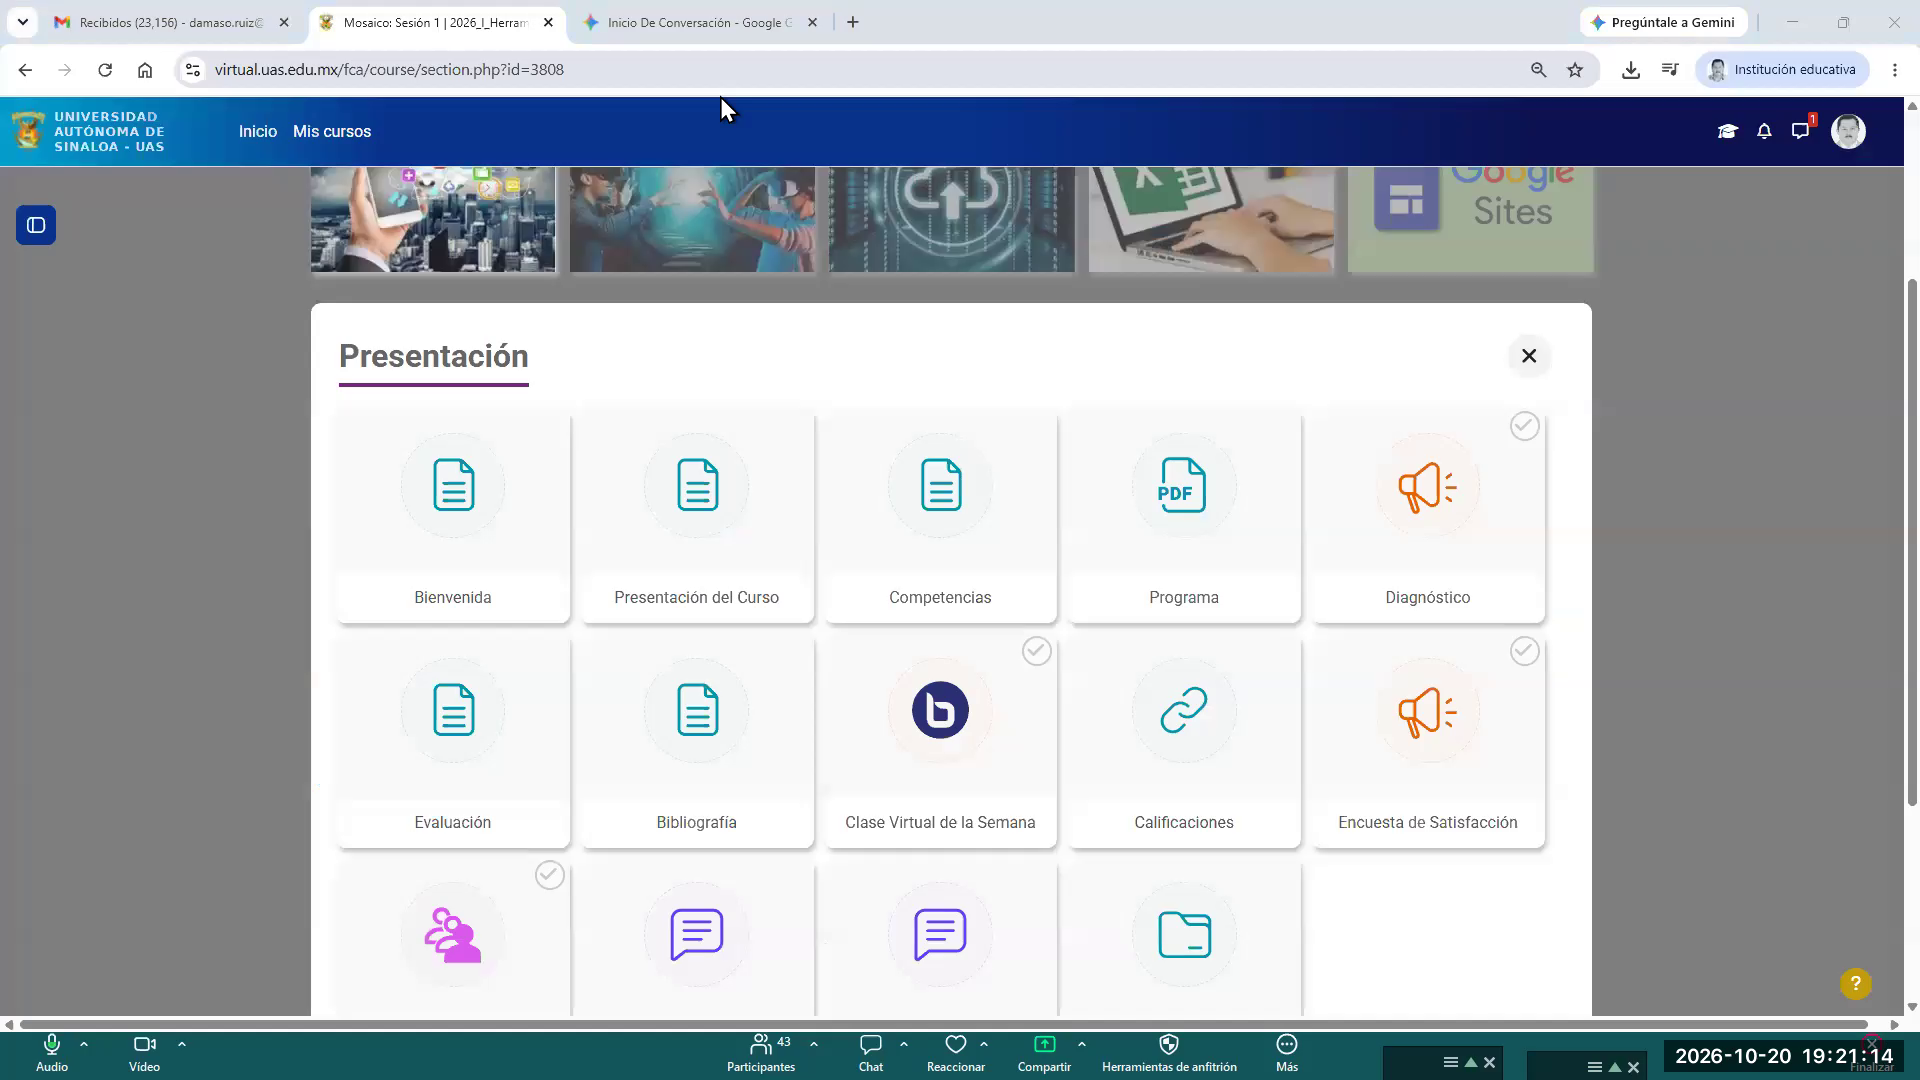
\includegraphics[width=0.88\linewidth]{referencias-herramientas-digitales/notas-herramientas-digitales/materiales-aula/capturas-clase/cap-01-s1-aula-virtual-encuadre-00-00-15.png}
  \caption{Evidencia visual de clase [00:00:15]: Vista general del aula virtual Moodle FCA UAS (Curso 635: 2026_I_Herramientas digitales_LCP) compartida por el Dr. Dámaso al inicio de la sesión. Fuente: Grabación docente UAS \cite{ruiz2026claseS1c1}.}
  \label{fig:uas-cap01-aula-virtual}
\end{figure}

% --- cap-02 [00:02:15] Módulos: 50144, 50147 ---
\begin{figure}[htbp]
  \centering
  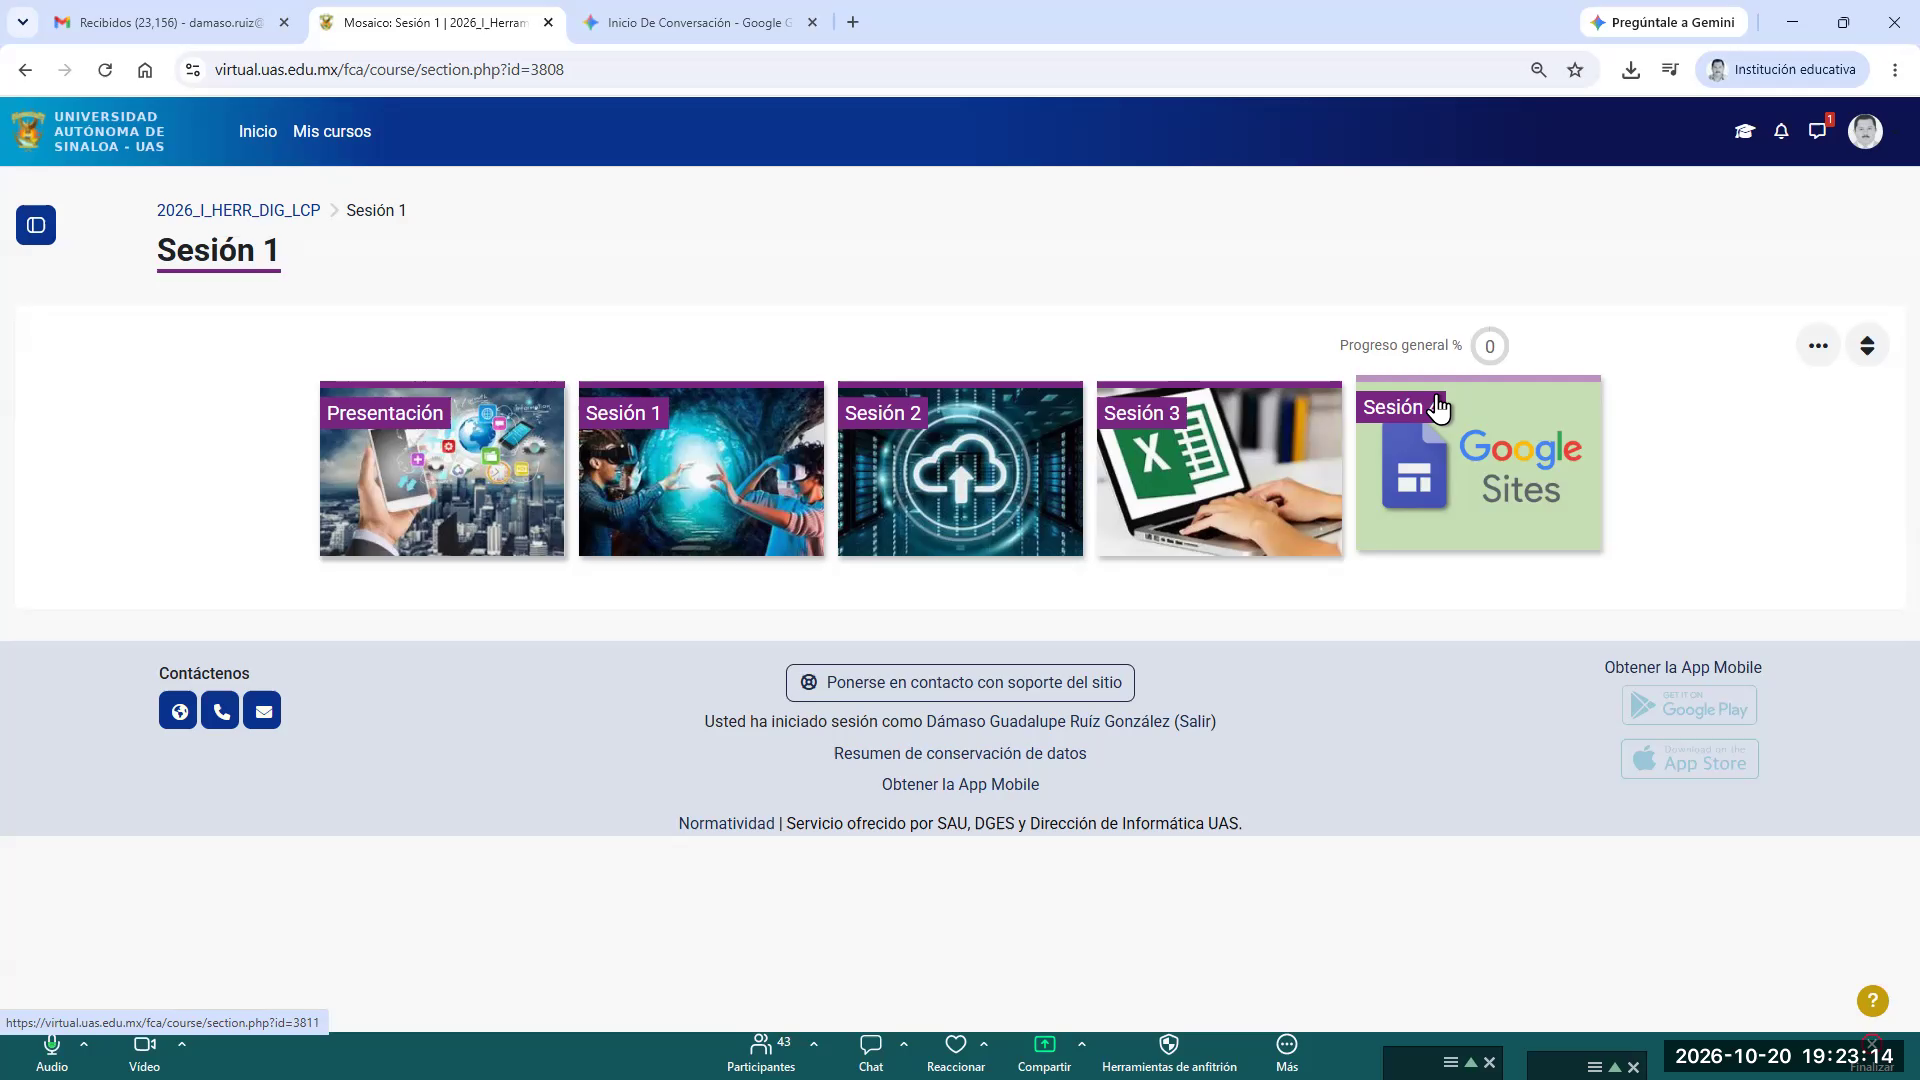
\includegraphics[width=0.88\linewidth]{referencias-herramientas-digitales/notas-herramientas-digitales/materiales-aula/capturas-clase/cap-02-s1-programa-google-sites-contabilidad-00-02-15.png}
  \caption{Evidencia visual de clase [00:02:15]: Presentación del temario general proyectando la Unidad 6 / Semana 4 (Diseño de páginas web con Google Sites y su articulación con Excel aplicado a la contaduría). Fuente: Grabación docente UAS \cite{ruiz2026claseS1c1}.}
  \label{fig:uas-cap02-programa-s4}
\end{figure}

% --- cap-03 [00:05:10] Módulos: 50102, 50107 ---
\begin{figure}[htbp]
  \centering
  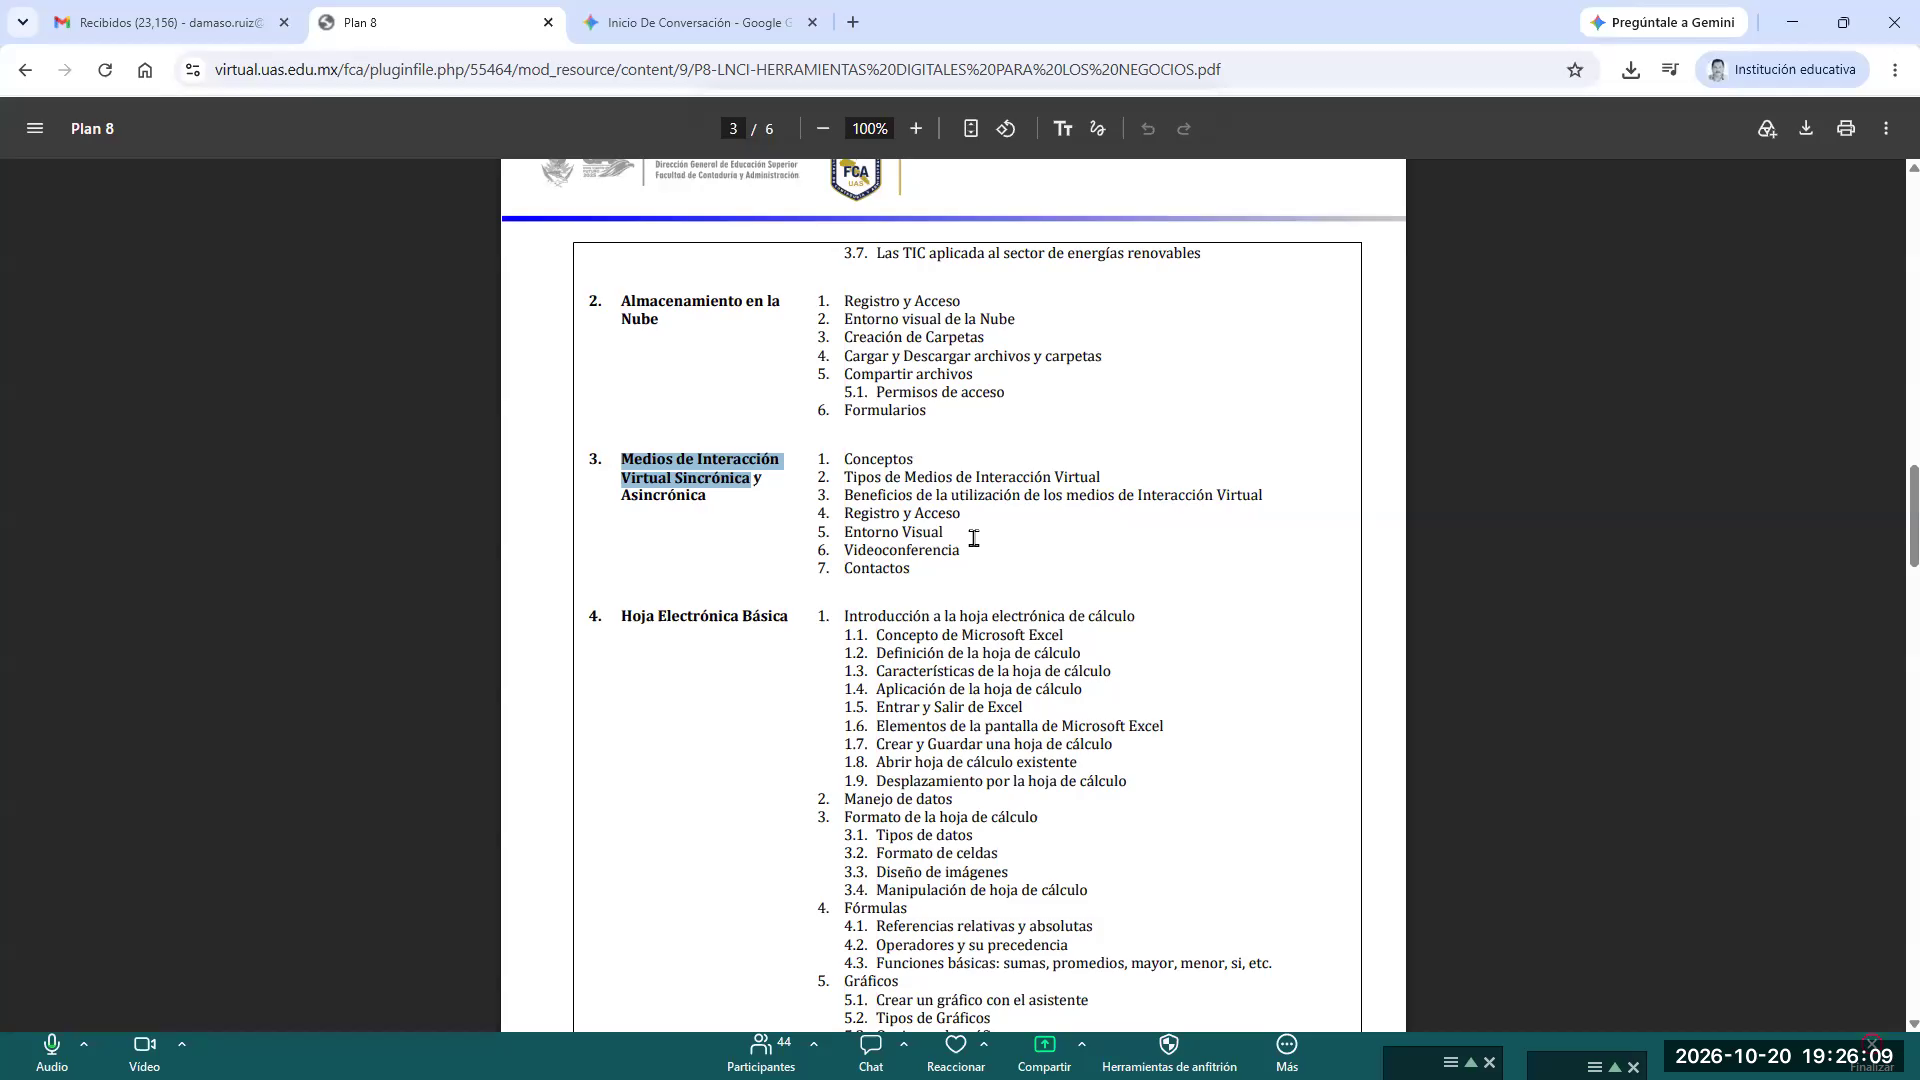
\includegraphics[width=0.88\linewidth]{referencias-herramientas-digitales/notas-herramientas-digitales/materiales-aula/capturas-clase/cap-03-s1-requisito-gmail-almacenamiento-nube-00-05-10.png}
  \caption{Evidencia visual de clase [00:05:10]: Sección de Almacenamiento en la Nube en plataforma UAS: directriz de cuenta obligatoria @gmail.com y política de envío directo en Moodle vs. enlace en Google Drive. Fuente: Grabación docente UAS \cite{ruiz2026claseS1c1}.}
  \label{fig:uas-cap03-regla-nube}
\end{figure}

% --- cap-04 [00:15:25] Módulos: 50085, 50103, 50114, 50130, 50131 ---
\begin{figure}[htbp]
  \centering
  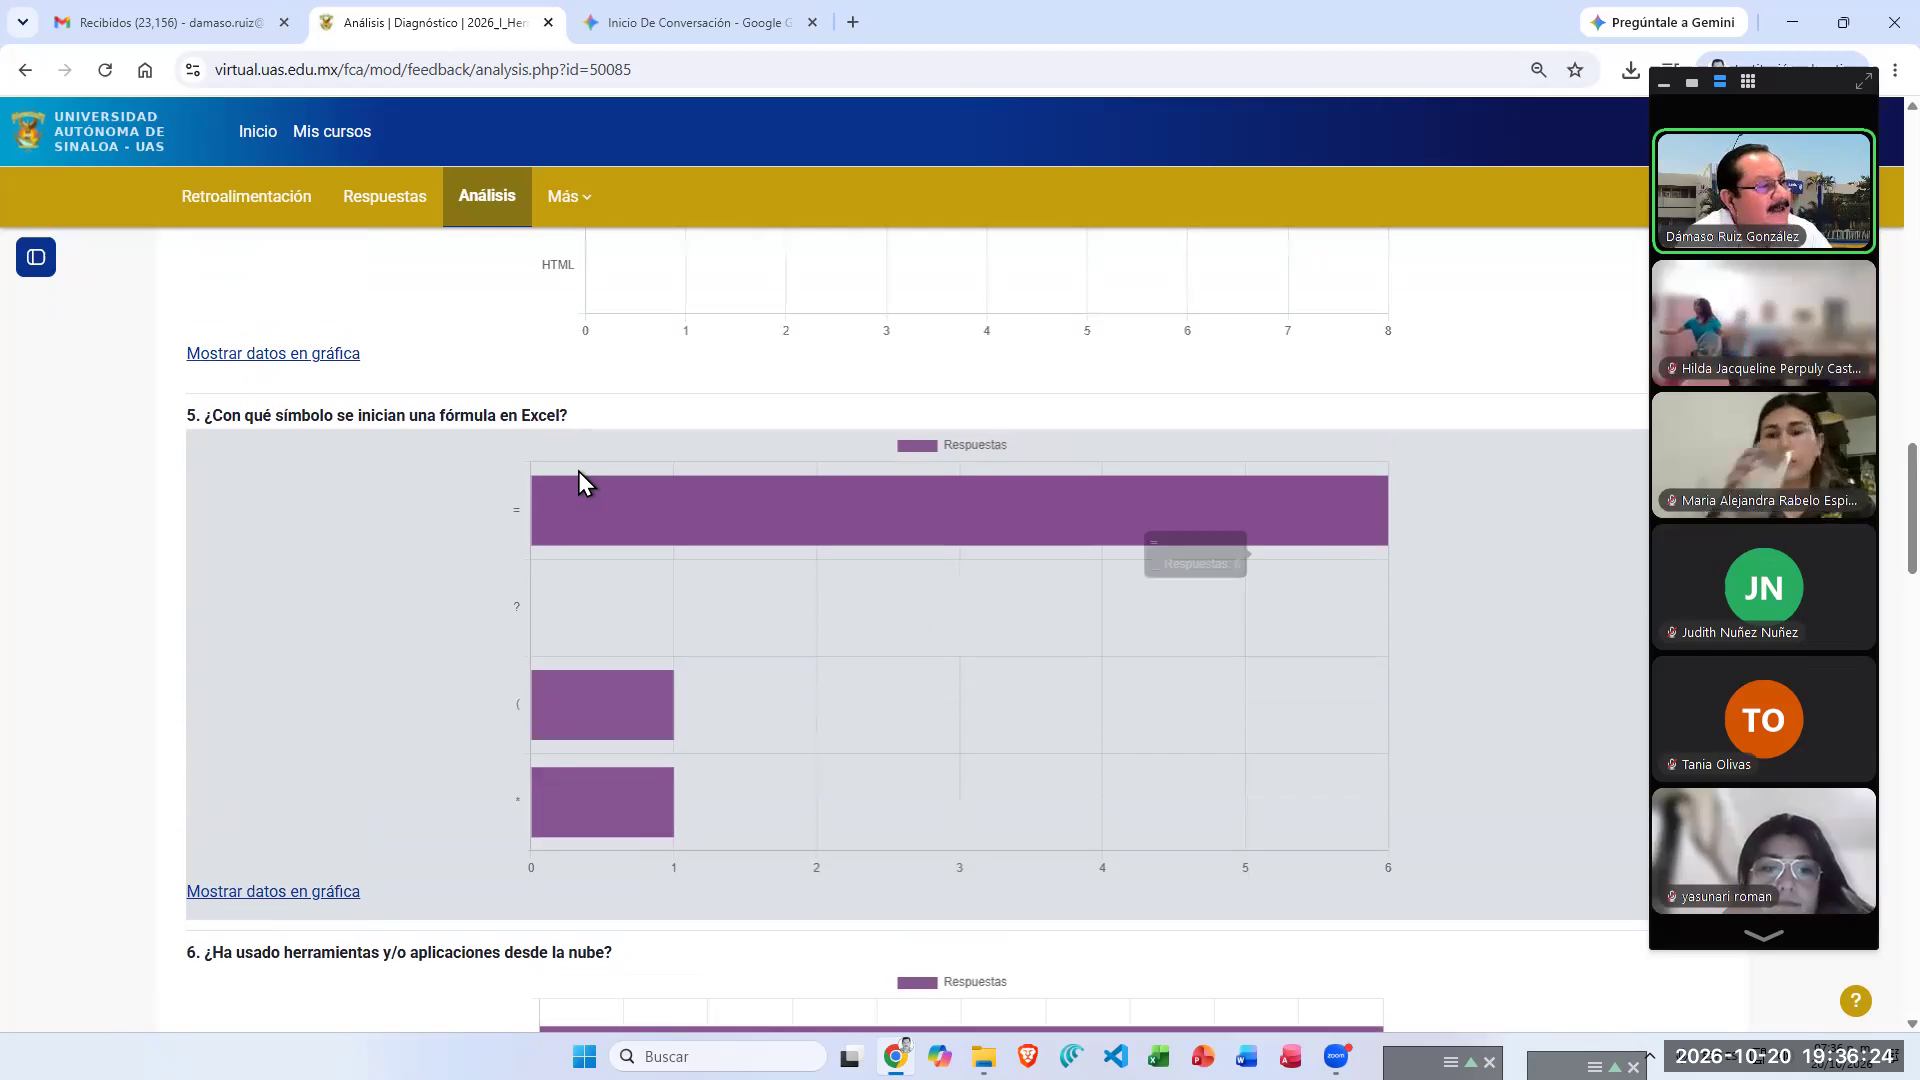
\includegraphics[width=0.88\linewidth]{referencias-herramientas-digitales/notas-herramientas-digitales/materiales-aula/capturas-clase/cap-04-s1-evaluacion-diagnostica-sintaxis-excel-00-15-25.png}
  \caption{Evidencia visual de clase [00:15:25]: Revisión en pantalla de las respuestas de la Evaluación Diagnóstica (módulo 50085) enfatizando la regla sintáctica de inicio de toda fórmula o función con '=' en Excel. Fuente: Grabación docente UAS \cite{ruiz2026claseS1c1}.}
  \label{fig:uas-cap04-diagnostico-excel}
\end{figure}

% --- cap-05 [00:17:05] Módulos: 50085, 50103, 50107, 50114 ---
\begin{figure}[htbp]
  \centering
  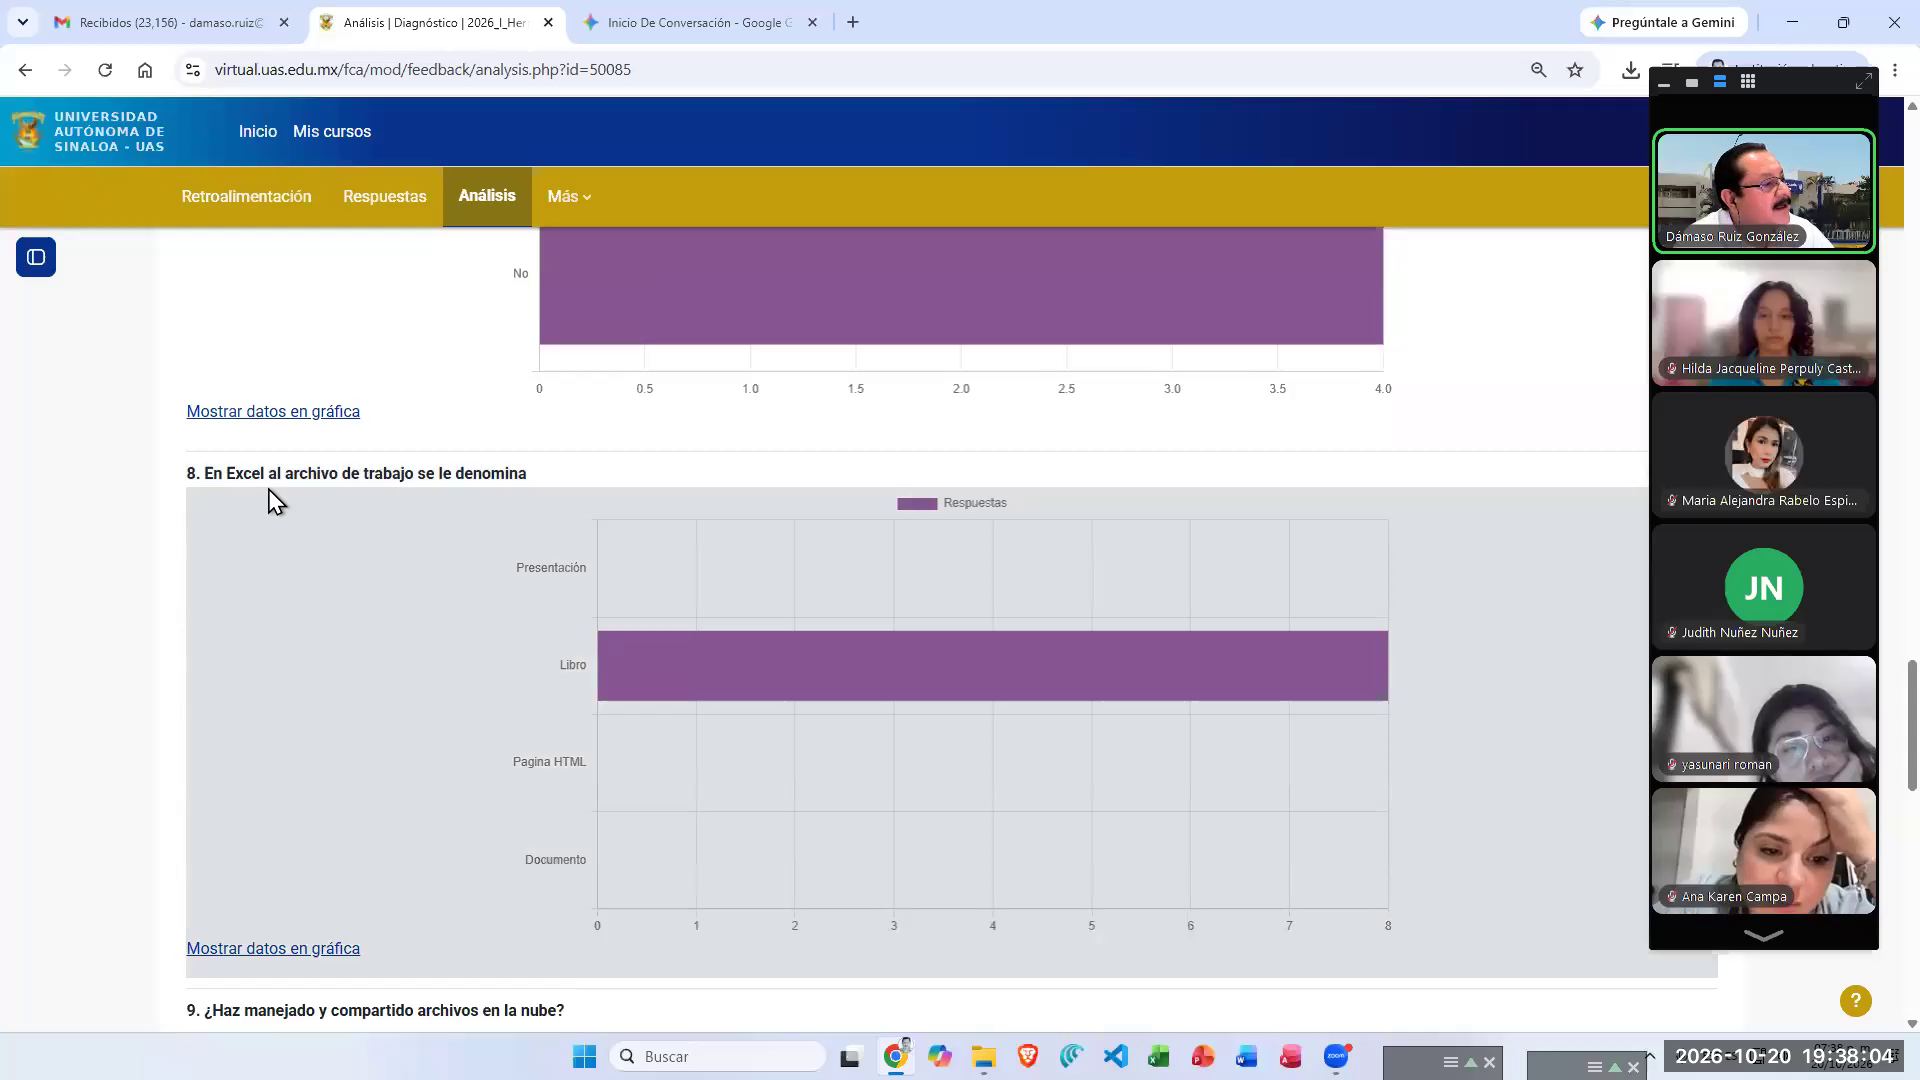
\includegraphics[width=0.88\linewidth]{referencias-herramientas-digitales/notas-herramientas-digitales/materiales-aula/capturas-clase/cap-05-s1-concepto-libro-excel-y-saas-nube-00-17-05.png}
  \caption{Evidencia visual de clase [00:17:05]: Análisis de reactivos diagnósticos sobre ejecución de aplicaciones en la nube (SaaS) y estructura jerárquica de archivos en Excel (Libro -> Hojas -> Celdas). Fuente: Grabación docente UAS \cite{ruiz2026claseS1c1}.}
  \label{fig:uas-cap05-libro-saas}
\end{figure}

% --- cap-06 [00:26:45] Módulos: 50102, 50103, 50113, 50114, 50130, 50131, 50144 ---
\begin{figure}[htbp]
  \centering
  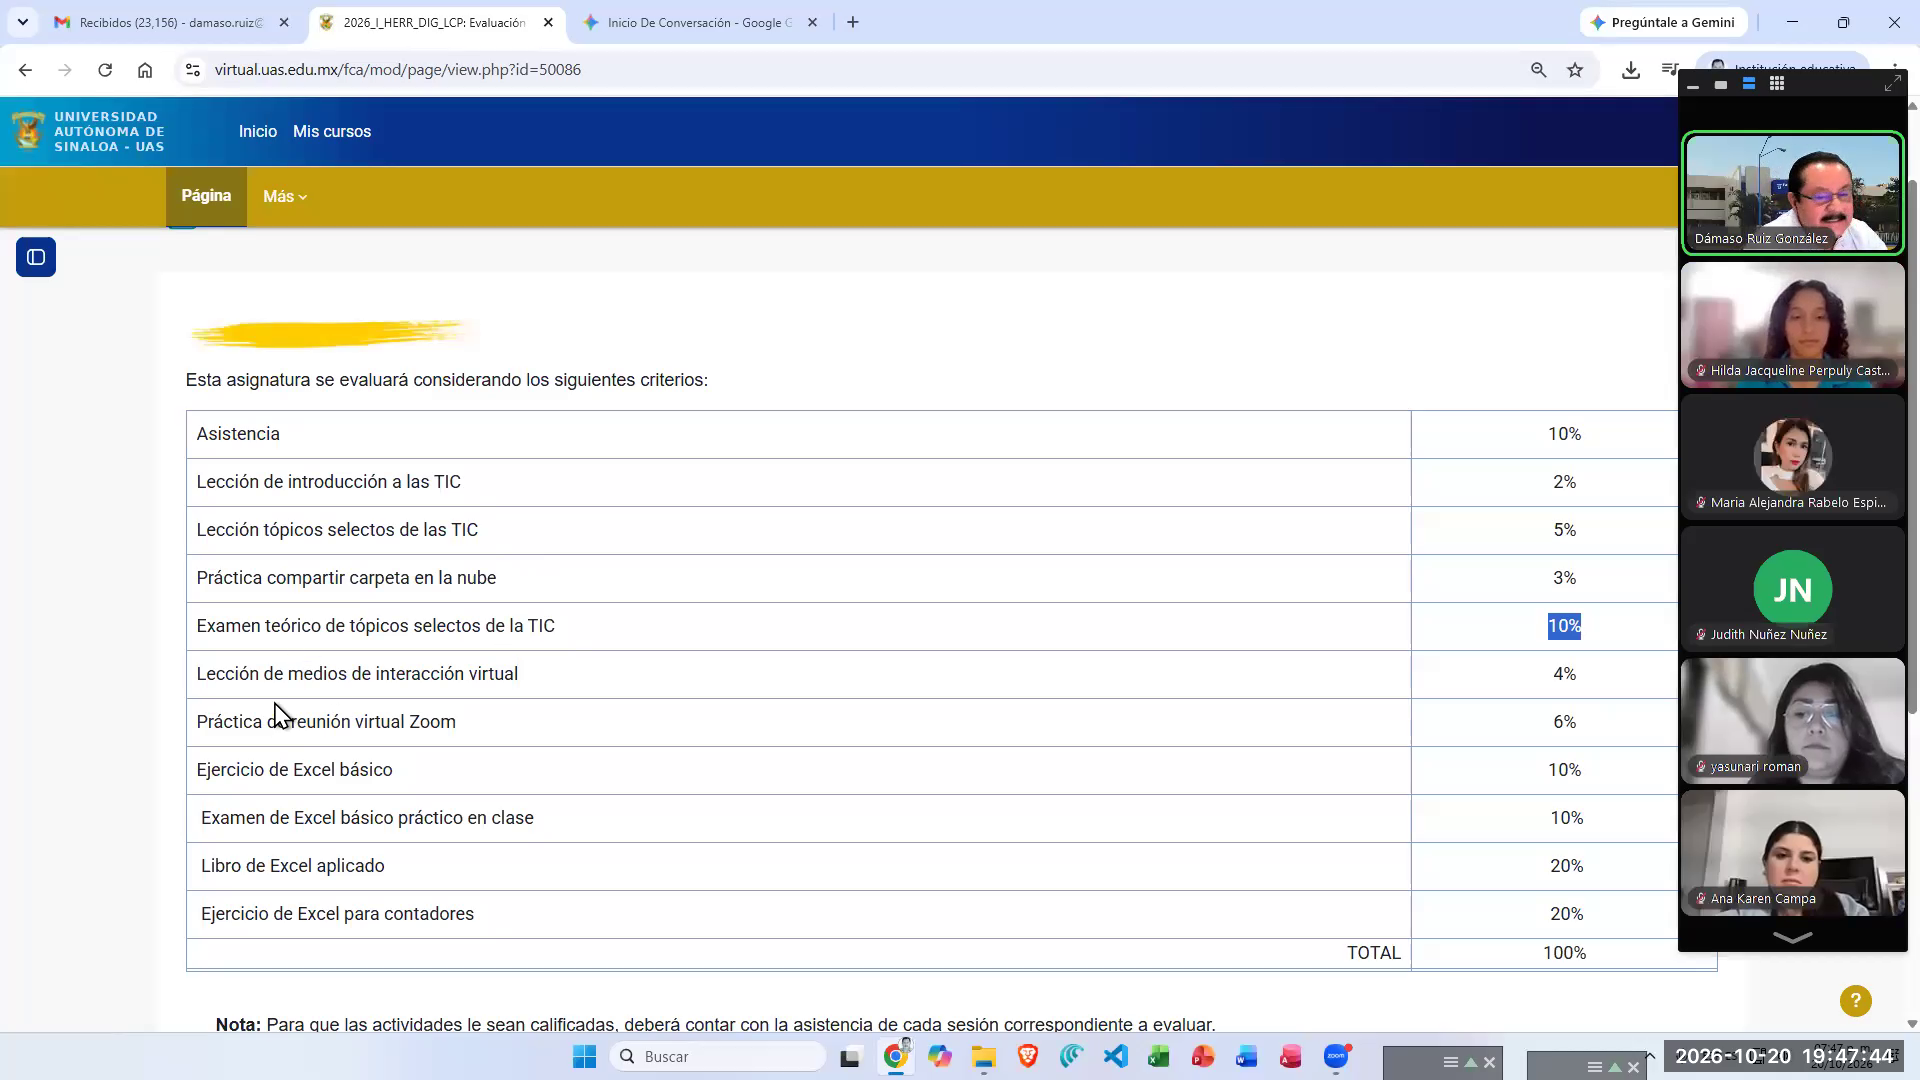
\includegraphics[width=0.88\linewidth]{referencias-herramientas-digitales/notas-herramientas-digitales/materiales-aula/capturas-clase/cap-06-s1-ponderacion-evaluacion-y-carpeta-apoyo-00-26-45.png}
  \caption{Evidencia visual de clase [00:26:45]: Tabla oficial de ponderación sumativa del curso (100%) y ubicación de la Carpeta de Apoyo (módulo 50094) con los ejercicios base obligatorios de las Sesiones 2 y 3. Fuente: Grabación docente UAS \cite{ruiz2026claseS1c1}.}
  \label{fig:uas-cap06-evaluacion-carpeta-apoyo}
\end{figure}

% --- cap-07 [00:31:50] Módulos: 50114, 50130, 50131 ---
\begin{figure}[htbp]
  \centering
  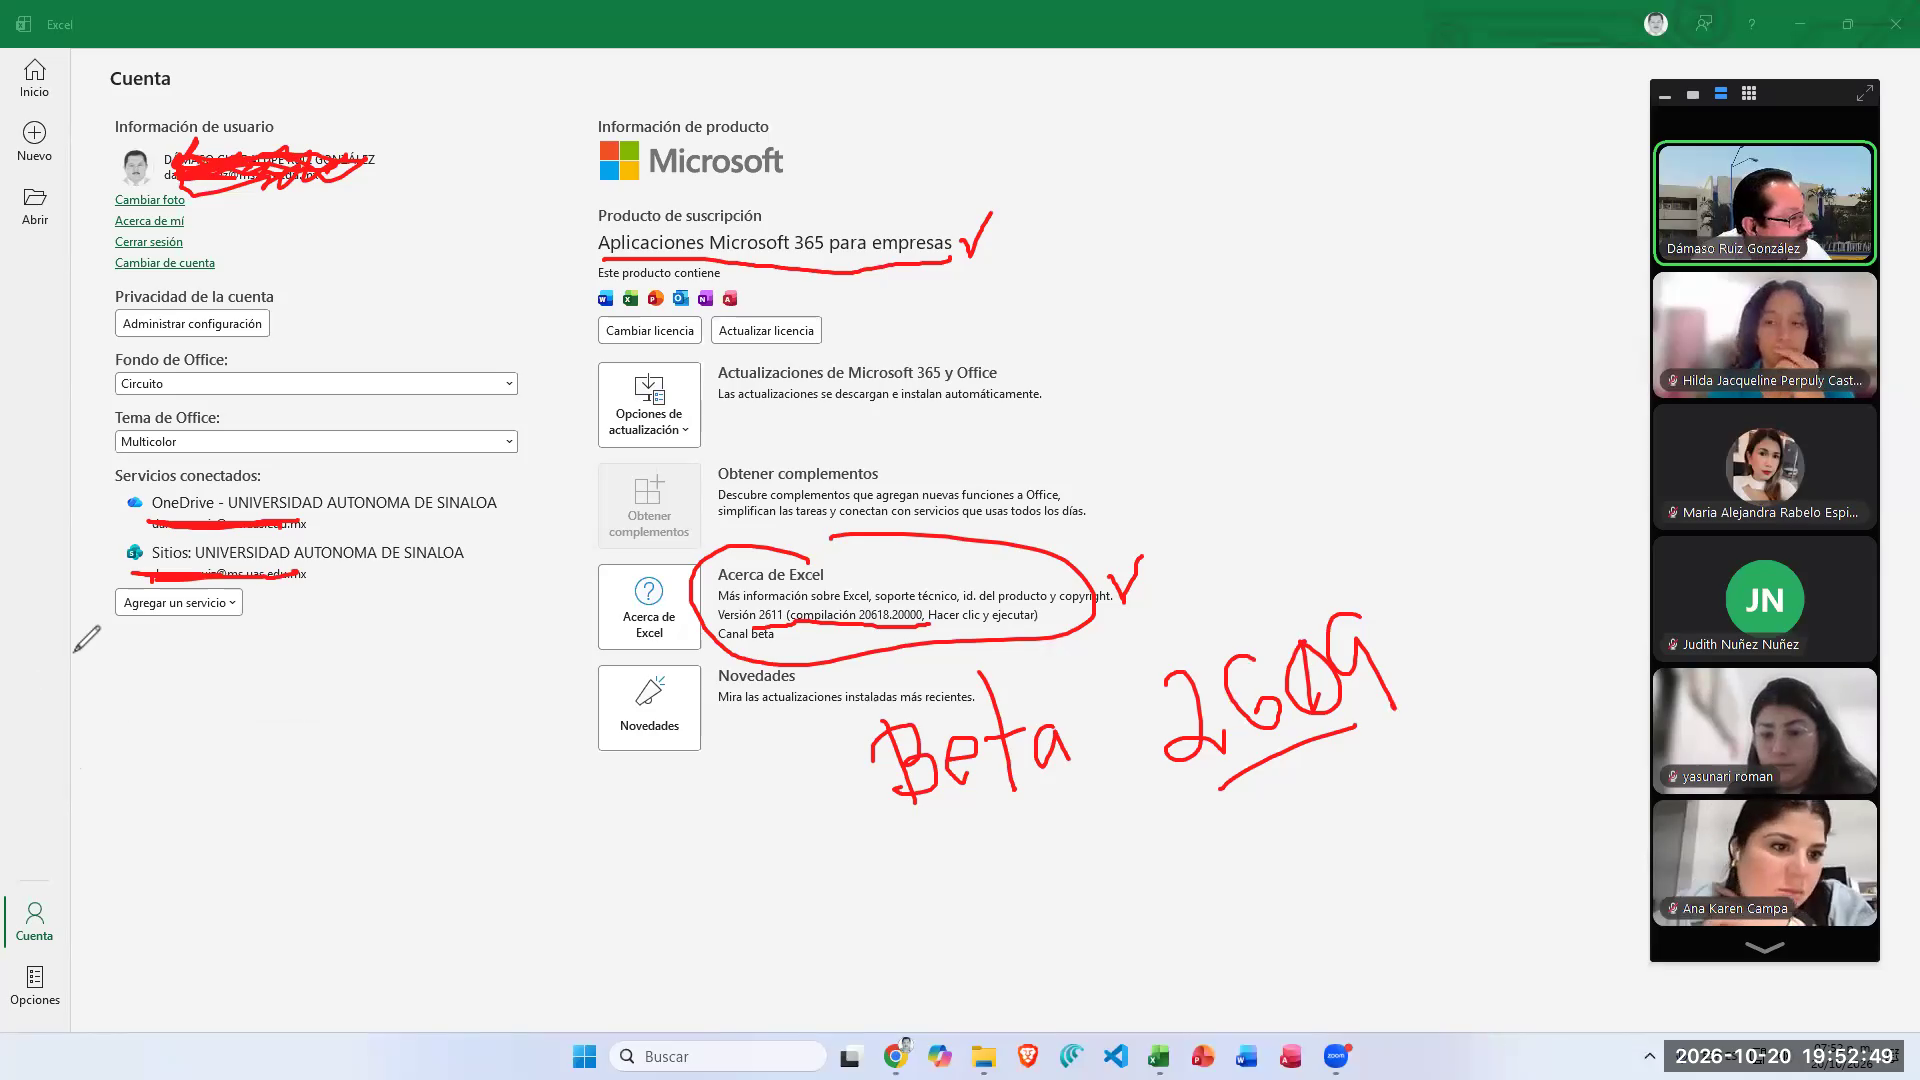
\includegraphics[width=0.88\linewidth]{referencias-herramientas-digitales/notas-herramientas-digitales/materiales-aula/capturas-clase/cap-07-s1-interfaz-excel-365-cuenta-version-00-31-50.png}
  \caption{Evidencia visual de clase [00:31:50]: Interfaz de Microsoft Excel 365 (menú Archivo -> Cuenta) proyectada en vivo para verificar la versión instalada y la licencia institucional @ms.uas.edu.mx. Fuente: Grabación docente UAS \cite{ruiz2026claseS1c1}.}
  \label{fig:uas-cap07-excel365-cuenta}
\end{figure}

% --- cap-08 [00:42:25] Módulos: 50100, 50101, 50103 ---
\begin{figure}[htbp]
  \centering
  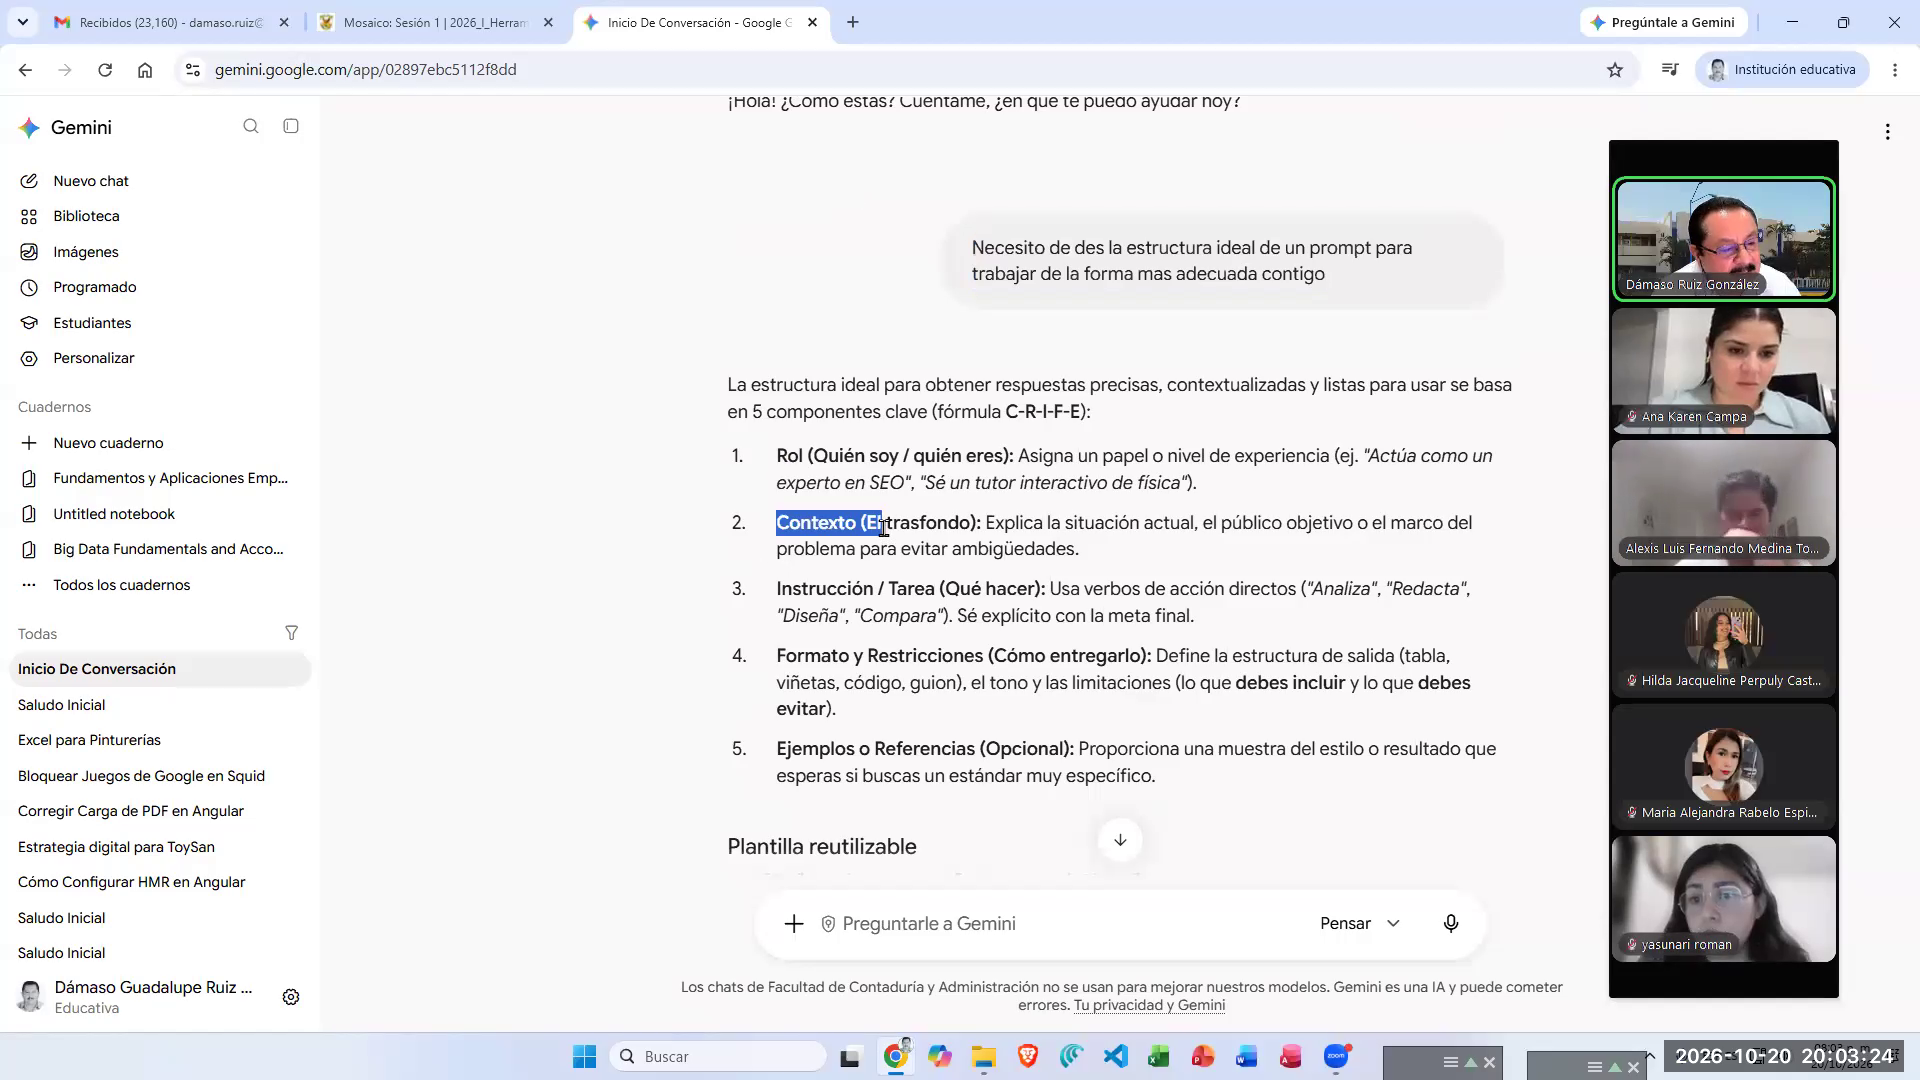
\includegraphics[width=0.88\linewidth]{referencias-herramientas-digitales/notas-herramientas-digitales/materiales-aula/capturas-clase/cap-08-s1-ingenieria-prompts-gemini-crifm-00-42-25.png}
  \caption{Evidencia visual de clase [00:42:25]: Demostración en vivo en Google Gemini de la estructura metodológica de un prompt profesional bajo la fórmula CRIFM (Contexto, Rol, Instrucción, Formato y Restricción). Fuente: Grabación docente UAS \cite{ruiz2026claseS1c1}.}
  \label{fig:uas-cap08-prompt-crifm}
\end{figure}

% --- cap-09 [00:46:35] Módulos: 50102, 50117 ---
\begin{figure}[htbp]
  \centering
  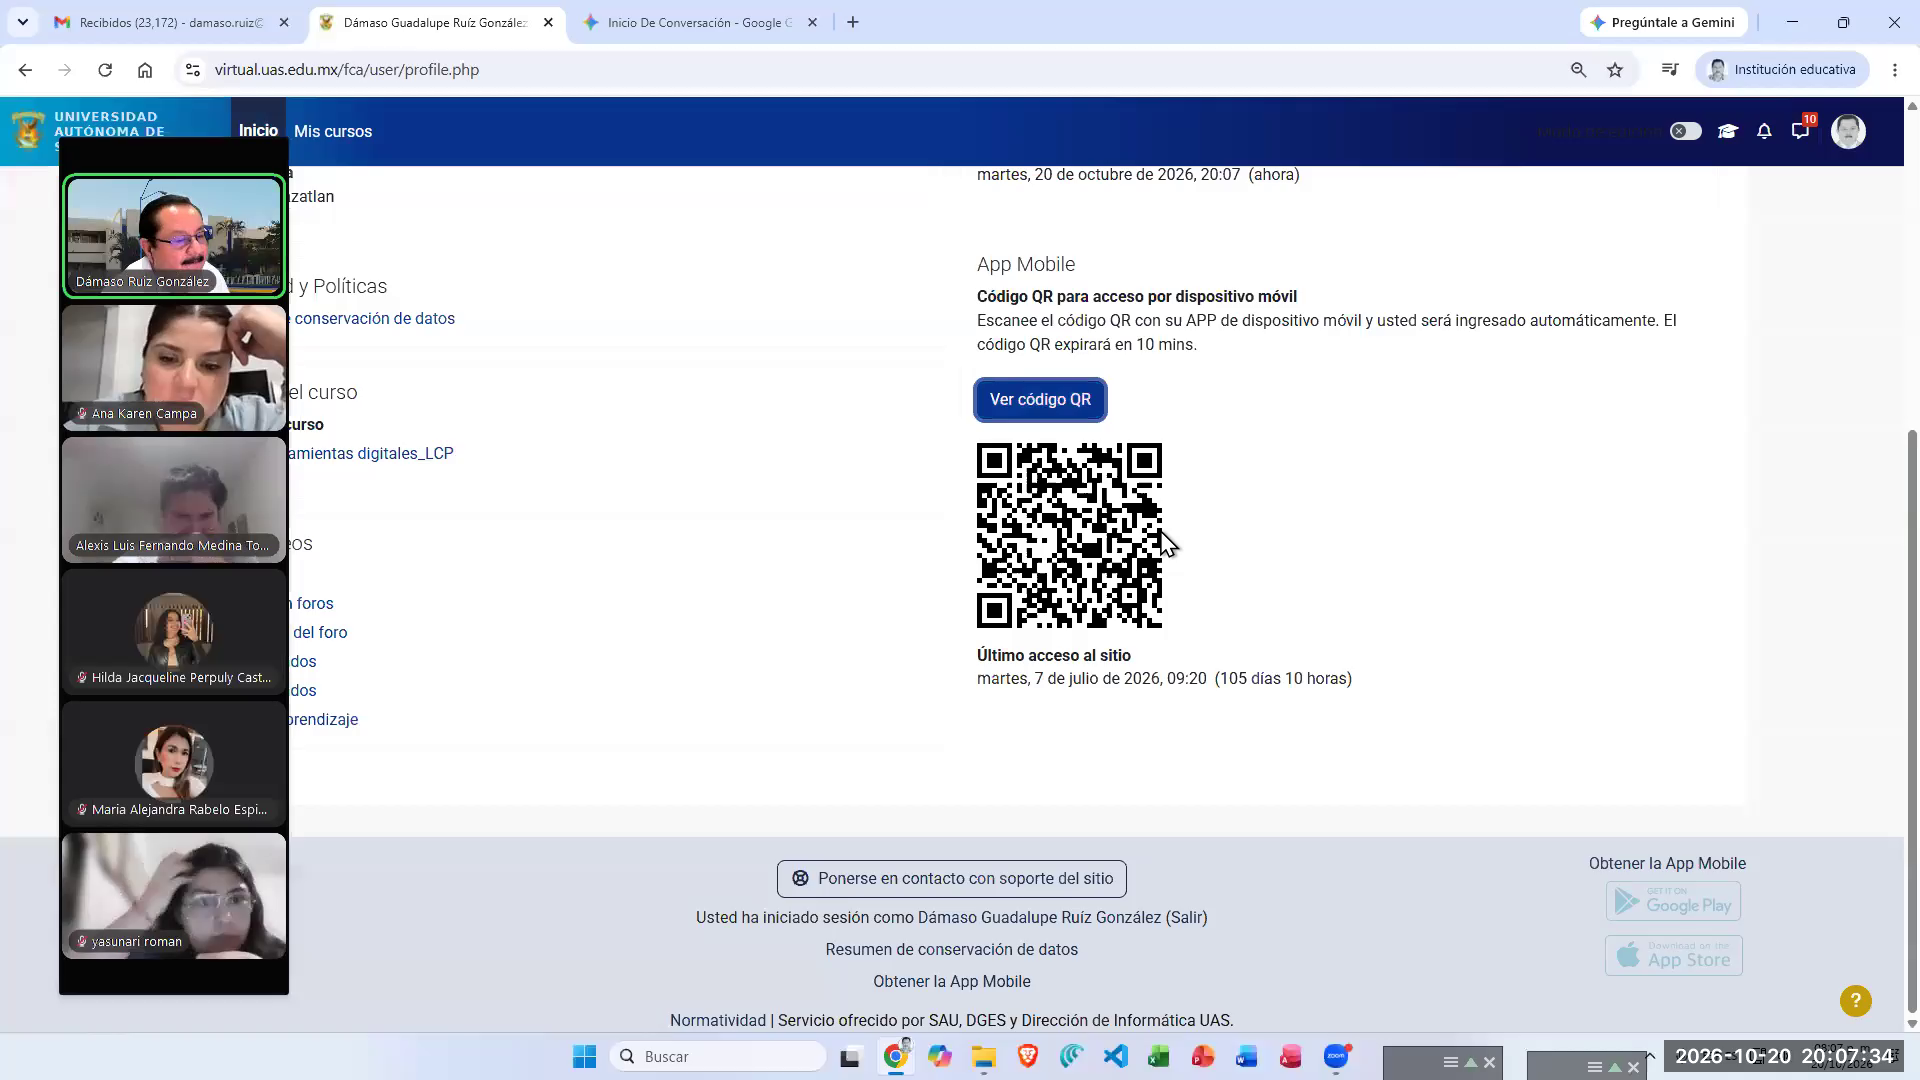
\includegraphics[width=0.88\linewidth]{referencias-herramientas-digitales/notas-herramientas-digitales/materiales-aula/capturas-clase/cap-09-s1-mensajeria-moodle-y-codigo-qr-movil-00-46-35.png}
  \caption{Evidencia visual de clase [00:46:35]: Demostración del sistema de mensajería interna de Moodle FCA UAS (canal oficial de envío de grabaciones) y código QR en el perfil para configurar Moodle Mobile. Fuente: Grabación docente UAS \cite{ruiz2026claseS1c1}.}
  \label{fig:uas-cap09-mensajeria-qr}
\end{figure}

% --- cap-10 [00:50:15] Módulos: 50102, 50107 ---
\begin{figure}[htbp]
  \centering
  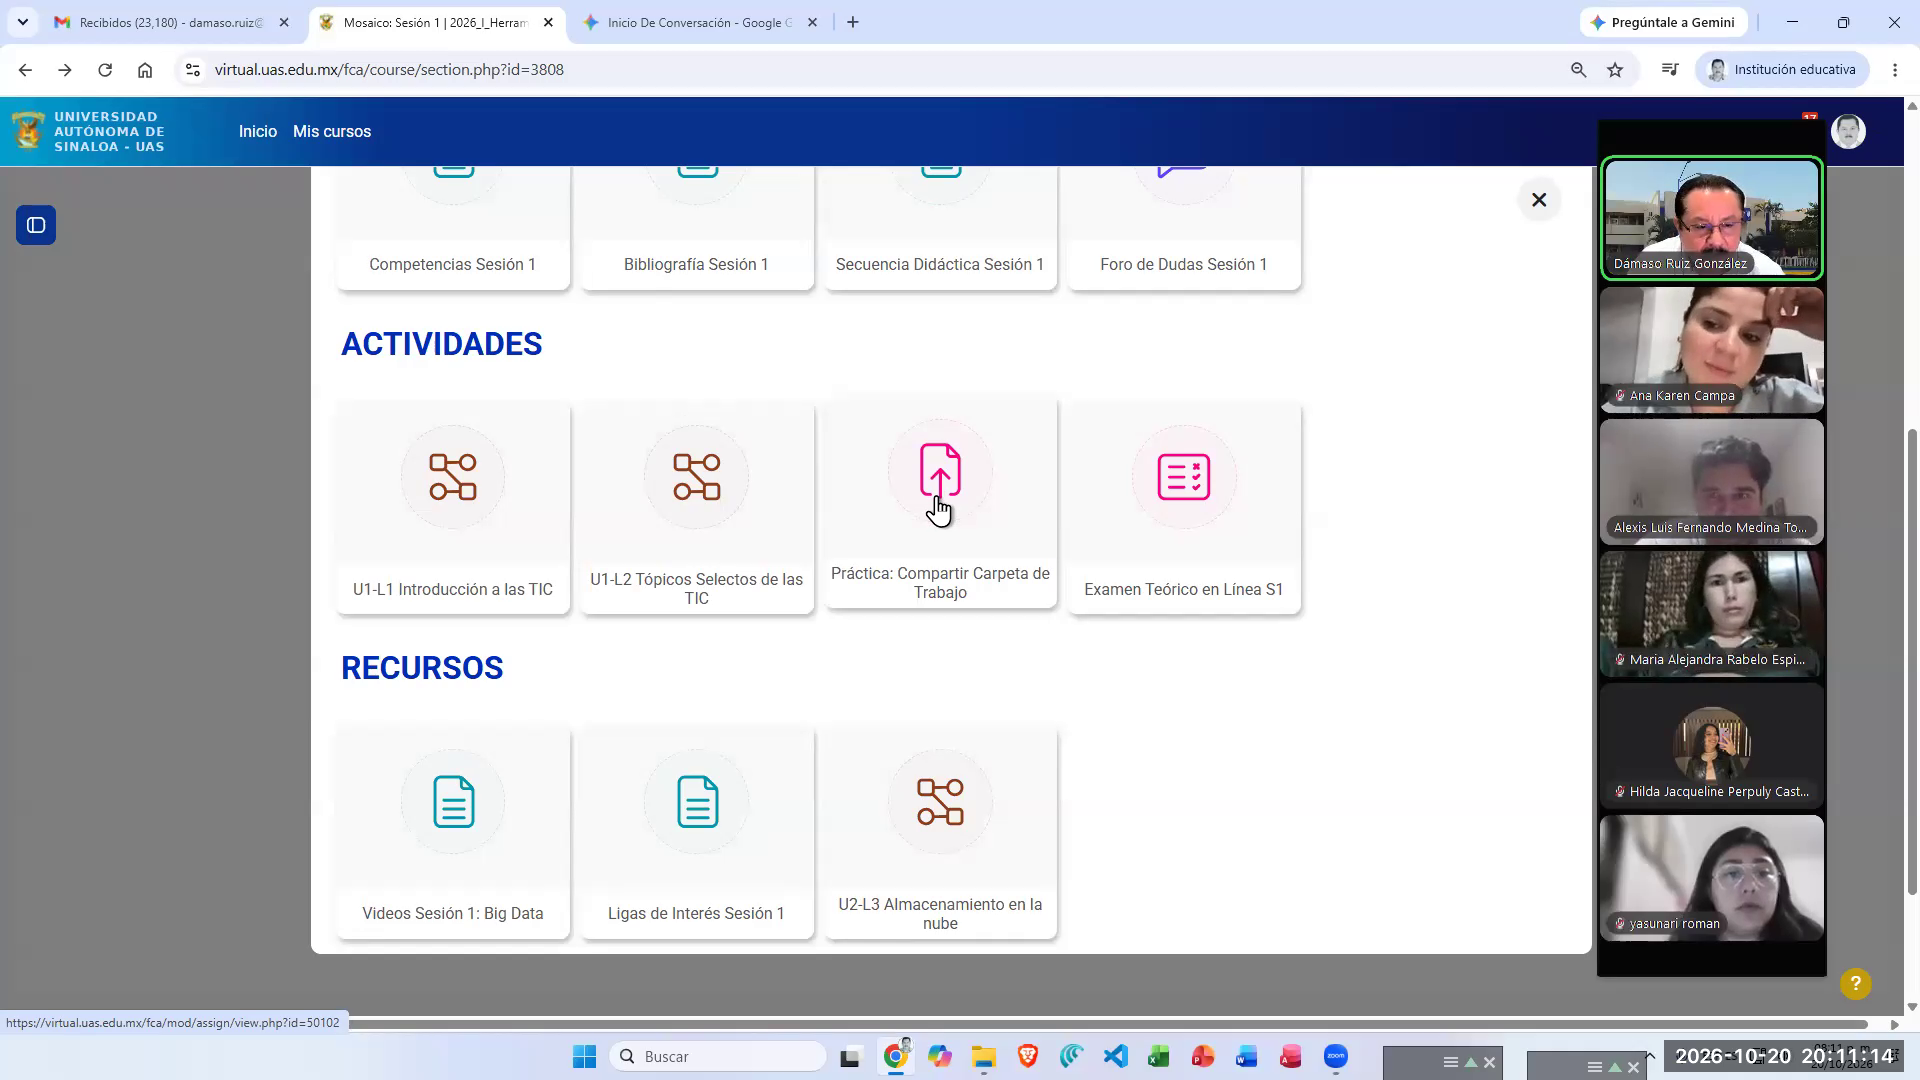
\includegraphics[width=0.88\linewidth]{referencias-herramientas-digitales/notas-herramientas-digitales/materiales-aula/capturas-clase/cap-10-s1-consigna-practica-compartir-carpeta-00-50-15.png}
  \caption{Evidencia visual de clase [00:50:15]: Explicación de la Práctica S1: Compartir Carpeta de Trabajo (módulo 50102), detallando nomenclatura 'GPO103 LCP - Nombre Apellido', compartición con el docente y respaldo documental. Fuente: Grabación docente UAS \cite{ruiz2026claseS1c1}.}
  \label{fig:uas-cap10-practica-carpeta}
\end{figure}

% --- cap-11 [00:56:15] Módulos: 50100, 50103 ---
\begin{figure}[htbp]
  \centering
  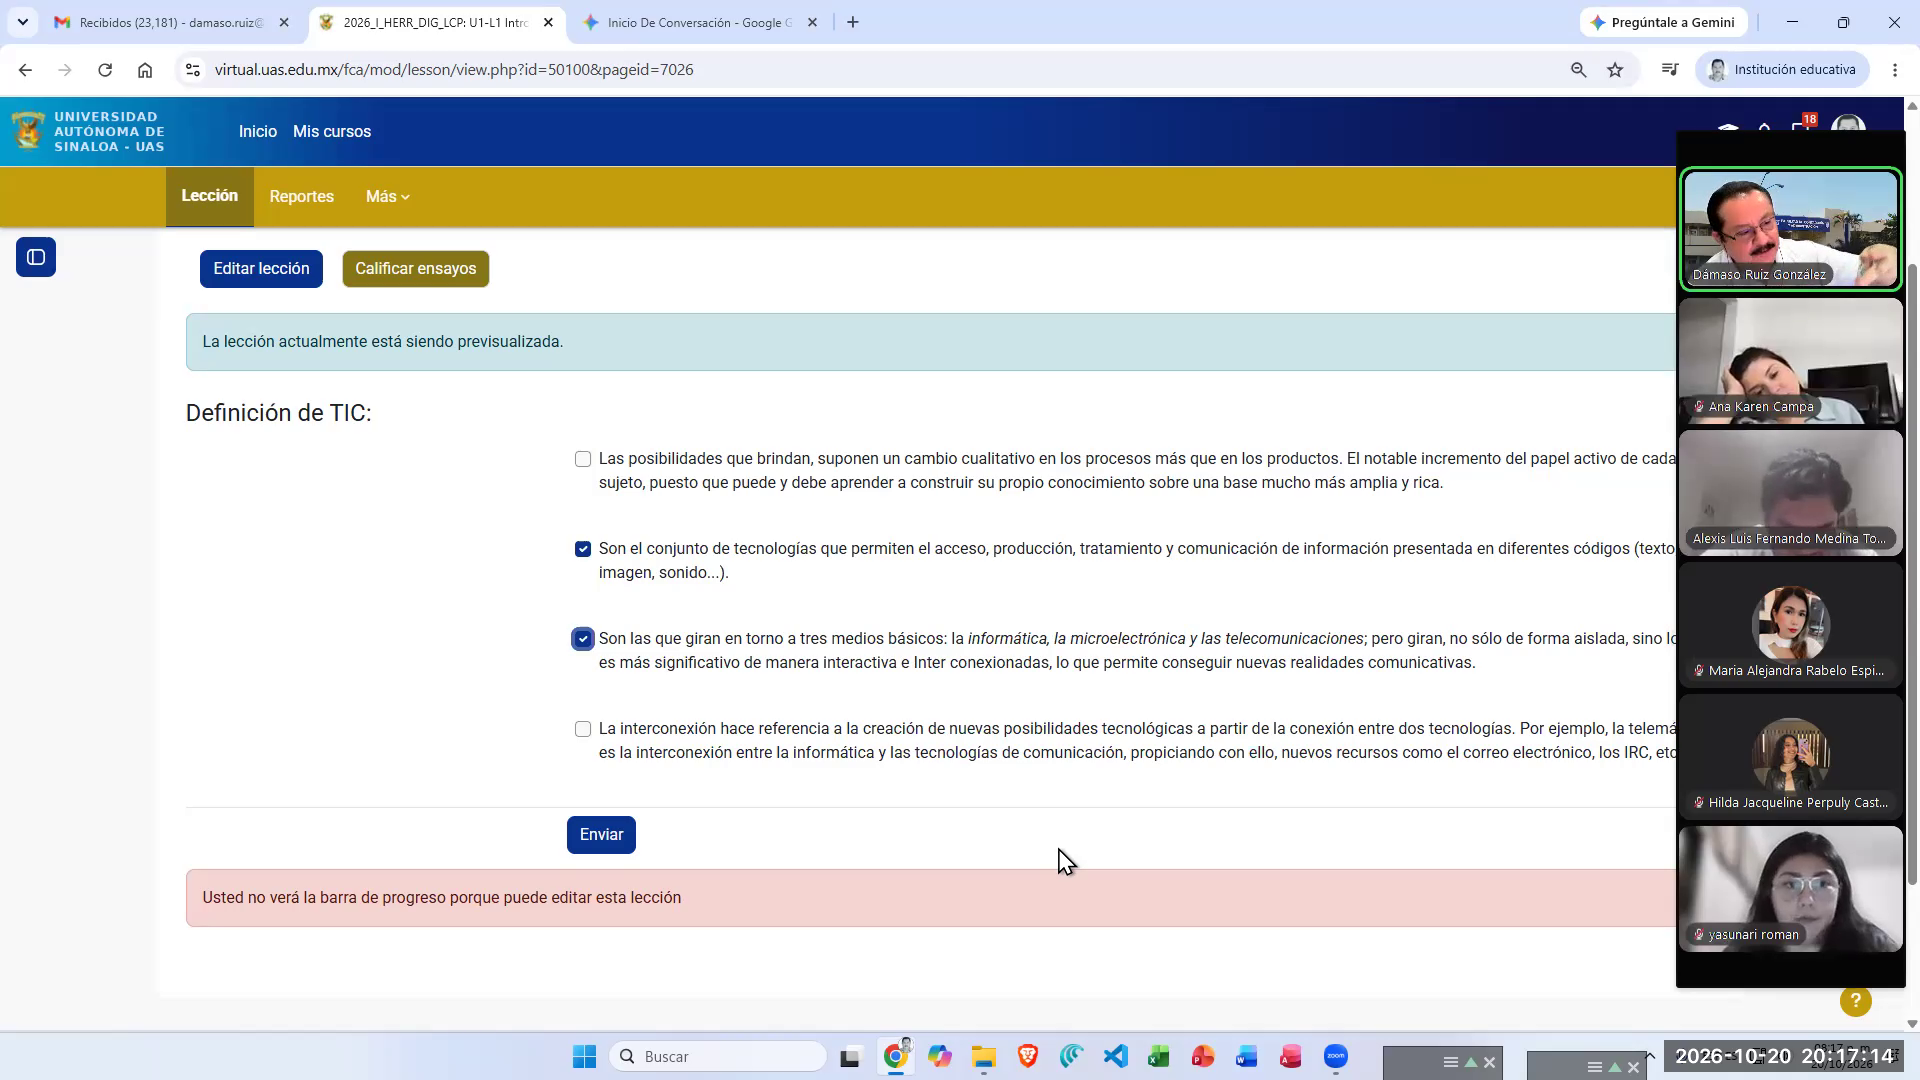
\includegraphics[width=0.88\linewidth]{referencias-herramientas-digitales/notas-herramientas-digitales/materiales-aula/capturas-clase/cap-11-s1-leccion-u1-l1-reactivos-tic-00-56-15.png}
  \caption{Evidencia visual de clase [00:56:15]: Recorrido interactivo por la Lección U1-L1 Introducción a las TIC (módulo 50100), mostrando la interfaz de preguntas aleatorias y el diferencial entre casillas cuadradas y botones de radio. Fuente: Grabación docente UAS \cite{ruiz2026claseS1c1}.}
  \label{fig:uas-cap11-leccion-u1l1}
\end{figure}

% --- cap-12 [01:04:10] Módulos: 50101, 50103 ---
\begin{figure}[htbp]
  \centering
  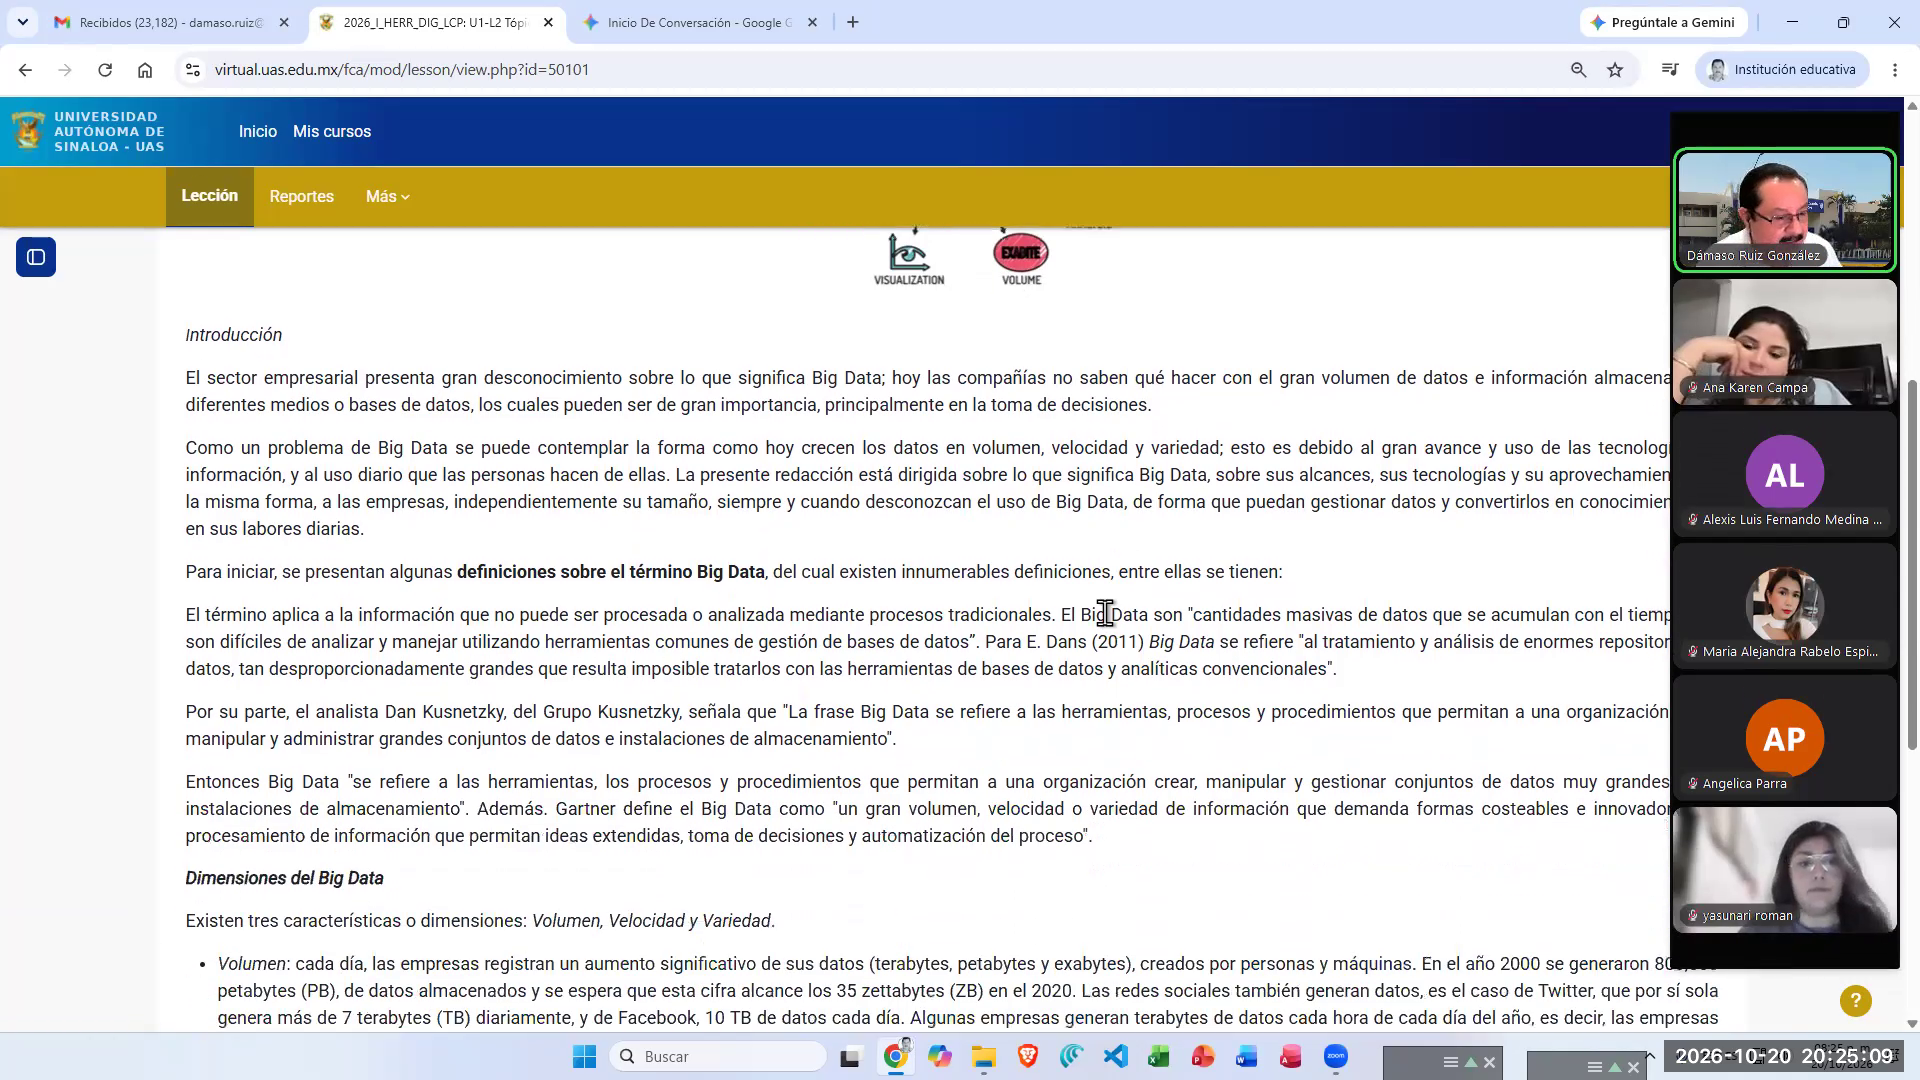
\includegraphics[width=0.88\linewidth]{referencias-herramientas-digitales/notas-herramientas-digitales/materiales-aula/capturas-clase/cap-12-s1-leccion-u1-l2-big-data-contabilidad-01-04-10.png}
  \caption{Evidencia visual de clase [01:04:10]: Proyección de la Lección U1-L2 Tópicos Selectos de las TIC: Big Data (módulo 50101), explicando las 3V y el cruce masivo de datos fiscales y comerciales (SAT, IMSS, retail). Fuente: Grabación docente UAS \cite{ruiz2026claseS1c1}.}
  \label{fig:uas-cap12-leccion-bigdata}
\end{figure}

% --- cap-13 [01:16:25] Módulos: 50101, 50103 ---
\begin{figure}[htbp]
  \centering
  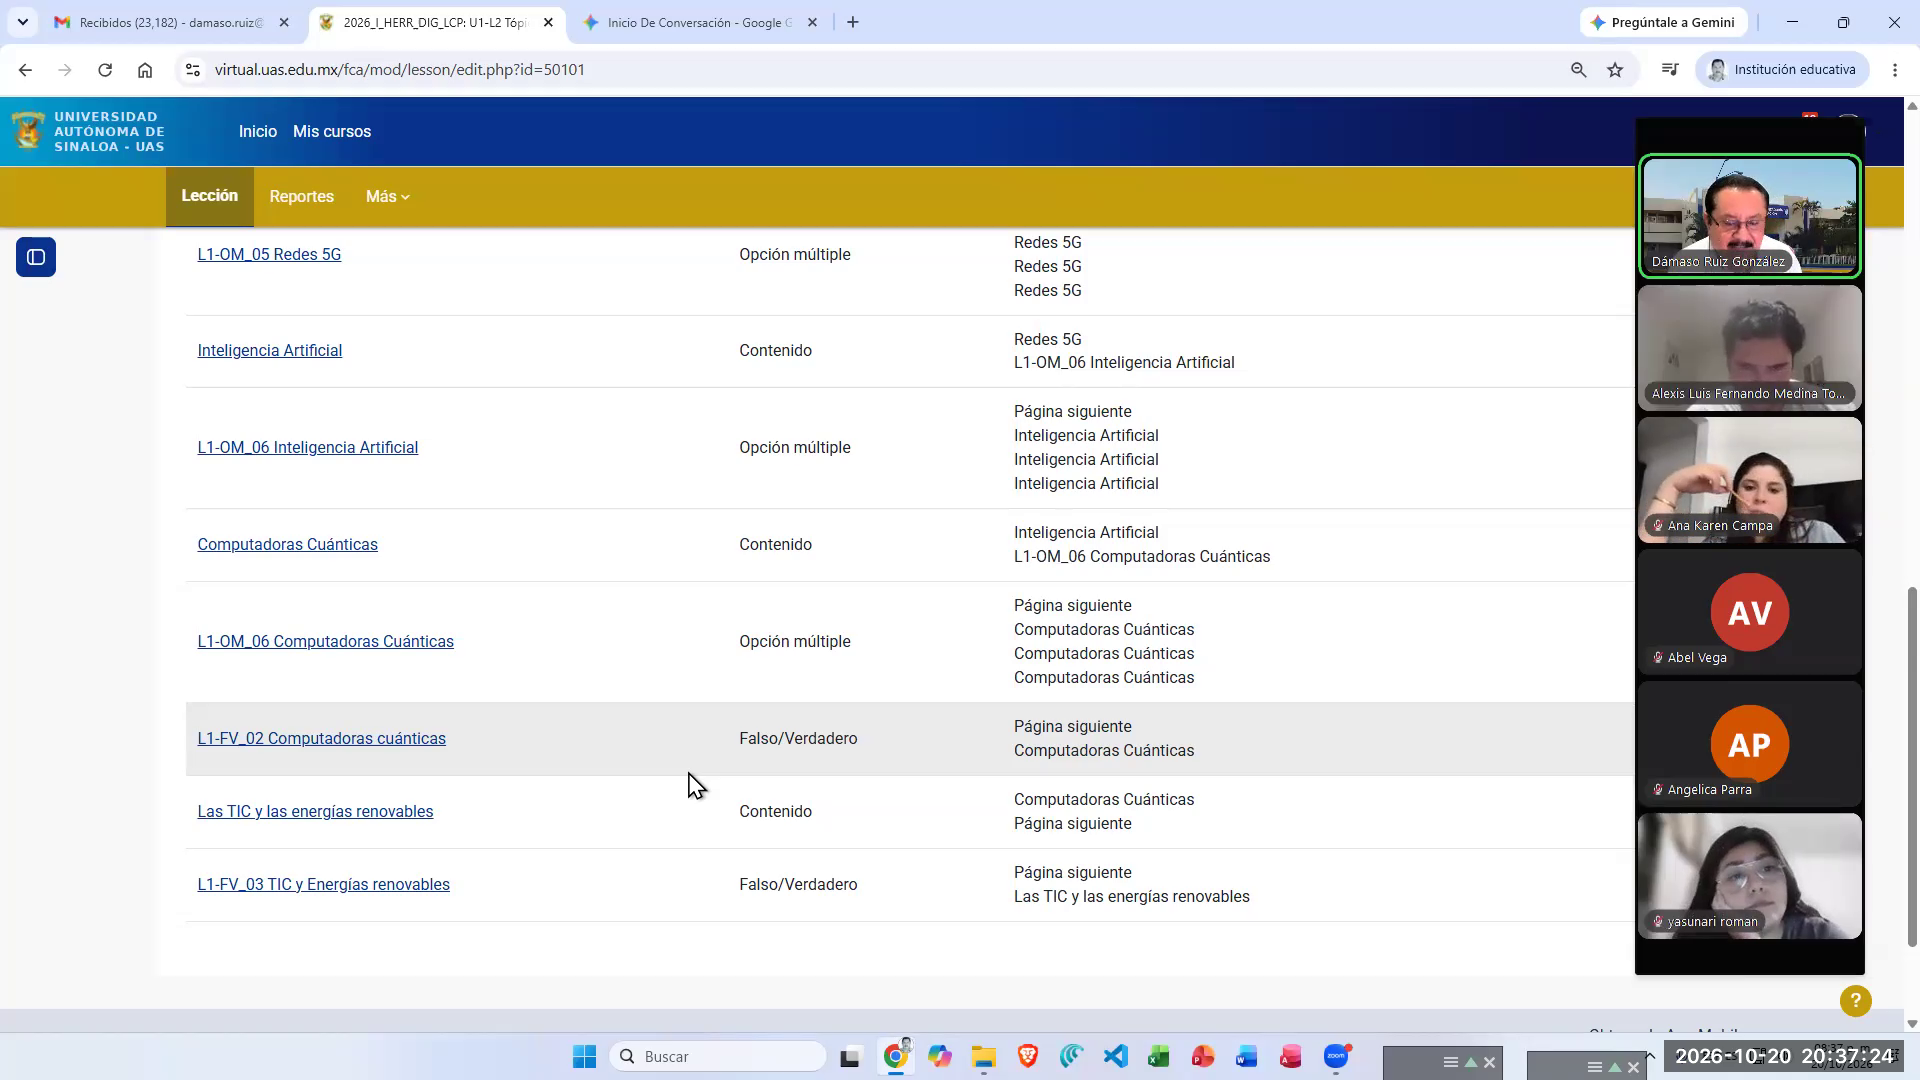
\includegraphics[width=0.88\linewidth]{referencias-herramientas-digitales/notas-herramientas-digitales/materiales-aula/capturas-clase/cap-13-s1-computacion-cuantica-superposicion-01-16-25.png}
  \caption{Evidencia visual de clase [01:16:25]: Sección de Computación Cuántica en U1-L2 (módulo 50101): contraste entre bits clásicos (0/1) y qubits en superposición, velocidad de procesamiento exponencial y riesgos criptográficos. Fuente: Grabación docente UAS \cite{ruiz2026claseS1c1}.}
  \label{fig:uas-cap13-computacion-cuantica}
\end{figure}

% --- cap-14 [01:24:45] Módulos: 50102, 50107 ---
\begin{figure}[htbp]
  \centering
  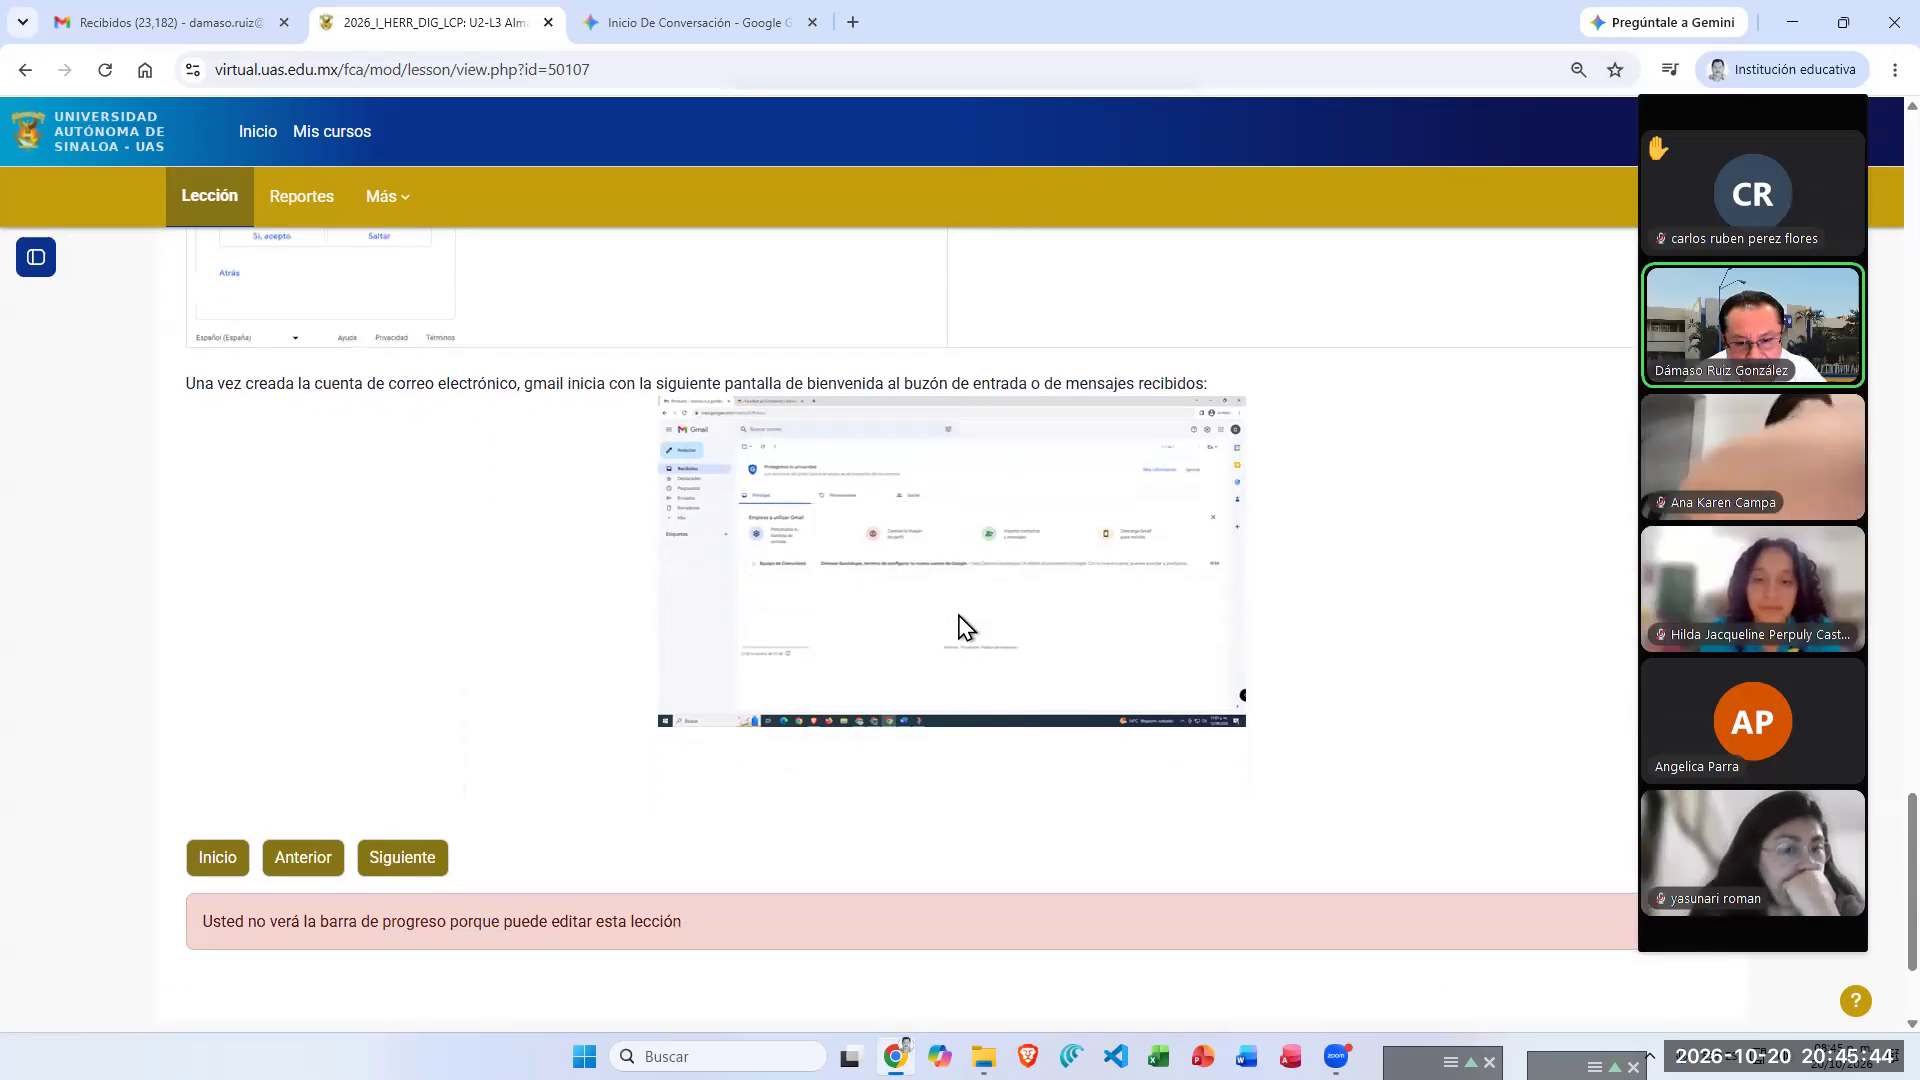
\includegraphics[width=0.88\linewidth]{referencias-herramientas-digitales/notas-herramientas-digitales/materiales-aula/capturas-clase/cap-14-s1-leccion-u2-l3-guia-google-drive-01-24-45.png}
  \caption{Evidencia visual de clase [01:24:45]: Demostración de cierre en la Lección U2-L3 Almacenamiento en la Nube (módulo 50107), exhibiendo el manual ilustrado para crear la carpeta en Google Drive y compartirla con el docente. Fuente: Grabación docente UAS \cite{ruiz2026claseS1c1}.}
  \label{fig:uas-cap14-leccion-u2l3-drive}
\end{figure}

% --- cap-15 [00:02:00] Módulos: 50113, 50118, 50114, 50130 ---
\begin{figure}[htbp]
  \centering
  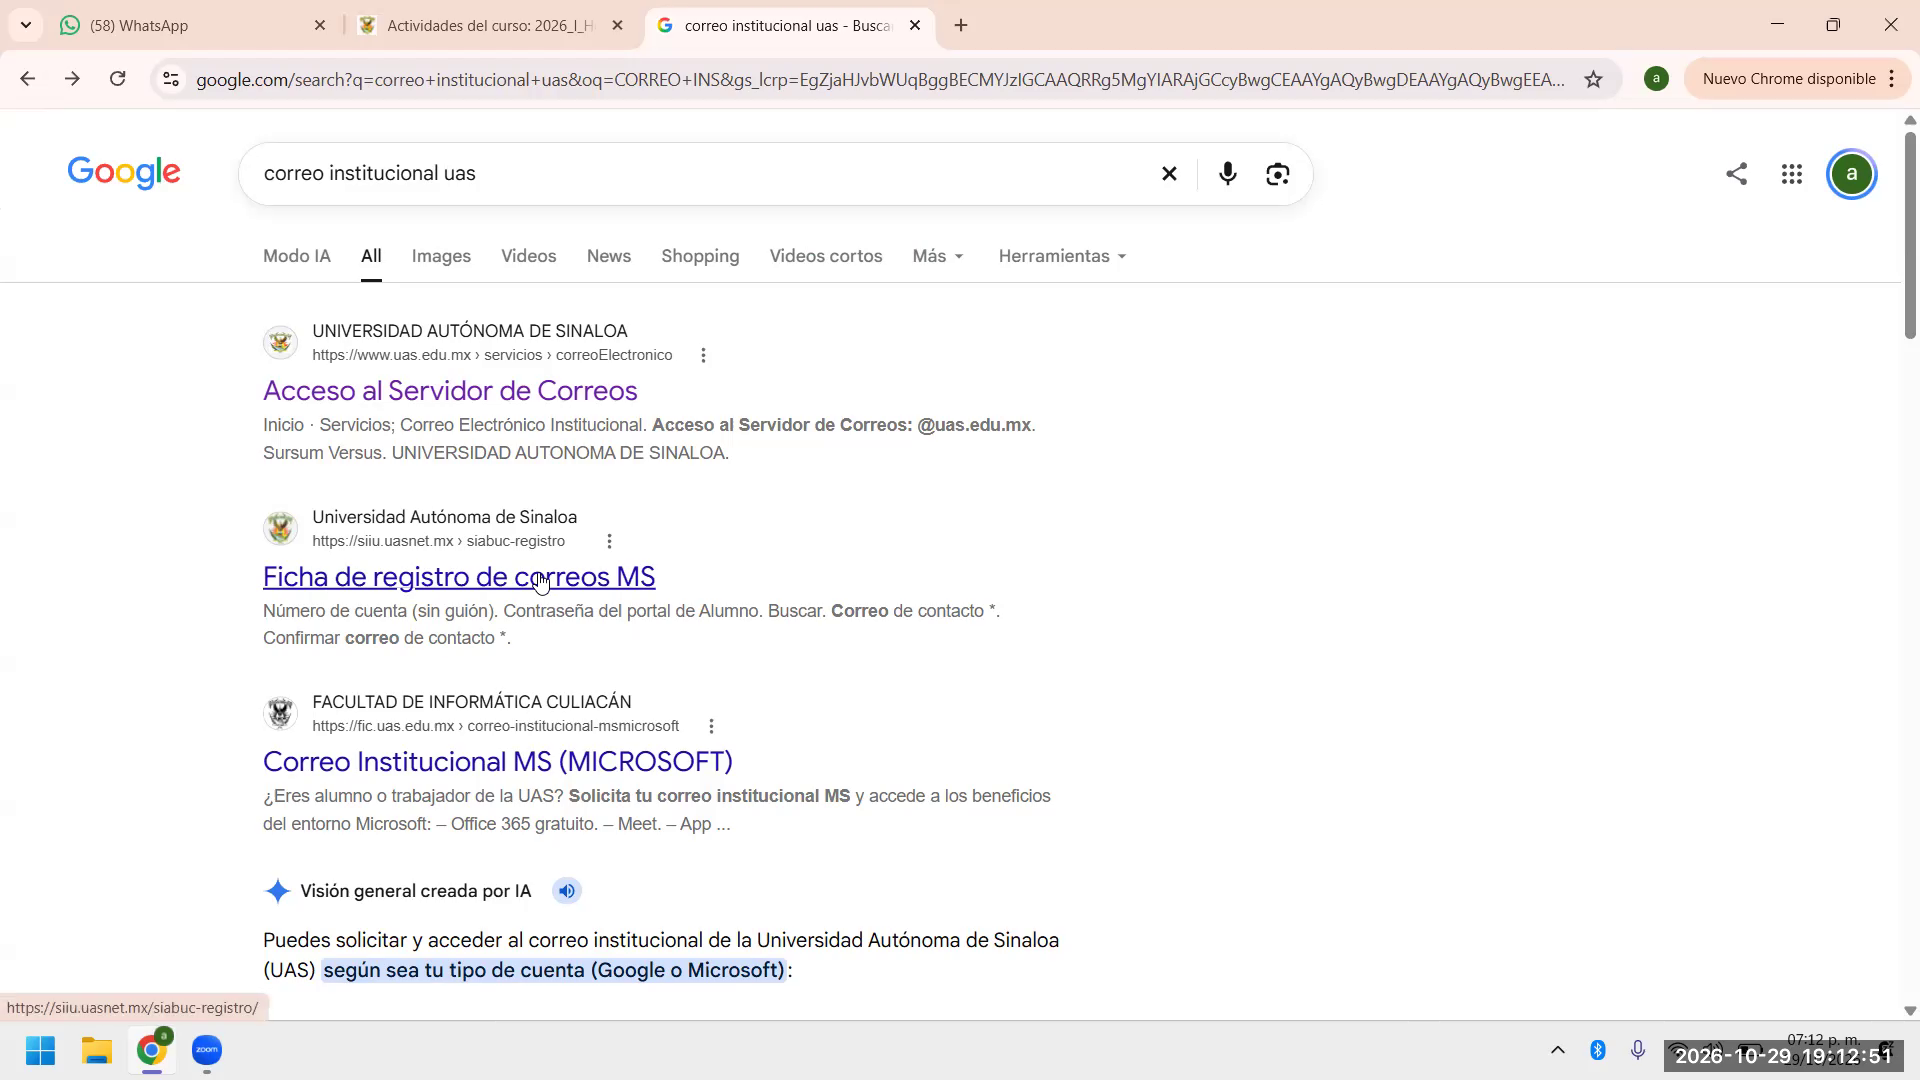
\includegraphics[width=0.88\linewidth]{referencias-herramientas-digitales/notas-herramientas-digitales/materiales-aula/capturas-clase/cap-15-s2-zoom-compartir-pantalla-y-correo-ms-00-02-00.png}
  \caption{Evidencia visual de clase [00:02:00]: Práctica real en vivo en Zoom durante la Sesión 2: una estudiante comparte pantalla desde Zoom guiada por el Dr. Dámaso para tramitar el correo institucional @ms.uas.edu.mx. Fuente: Grabación docente UAS \cite{ruiz2026claseS1c1}.}
  \label{fig:uas-cap15-zoom-compartir-pantalla}
\end{figure}

% --- cap-16 [00:21:15] Módulos: 50114, 50130, 50131 ---
\begin{figure}[htbp]
  \centering
  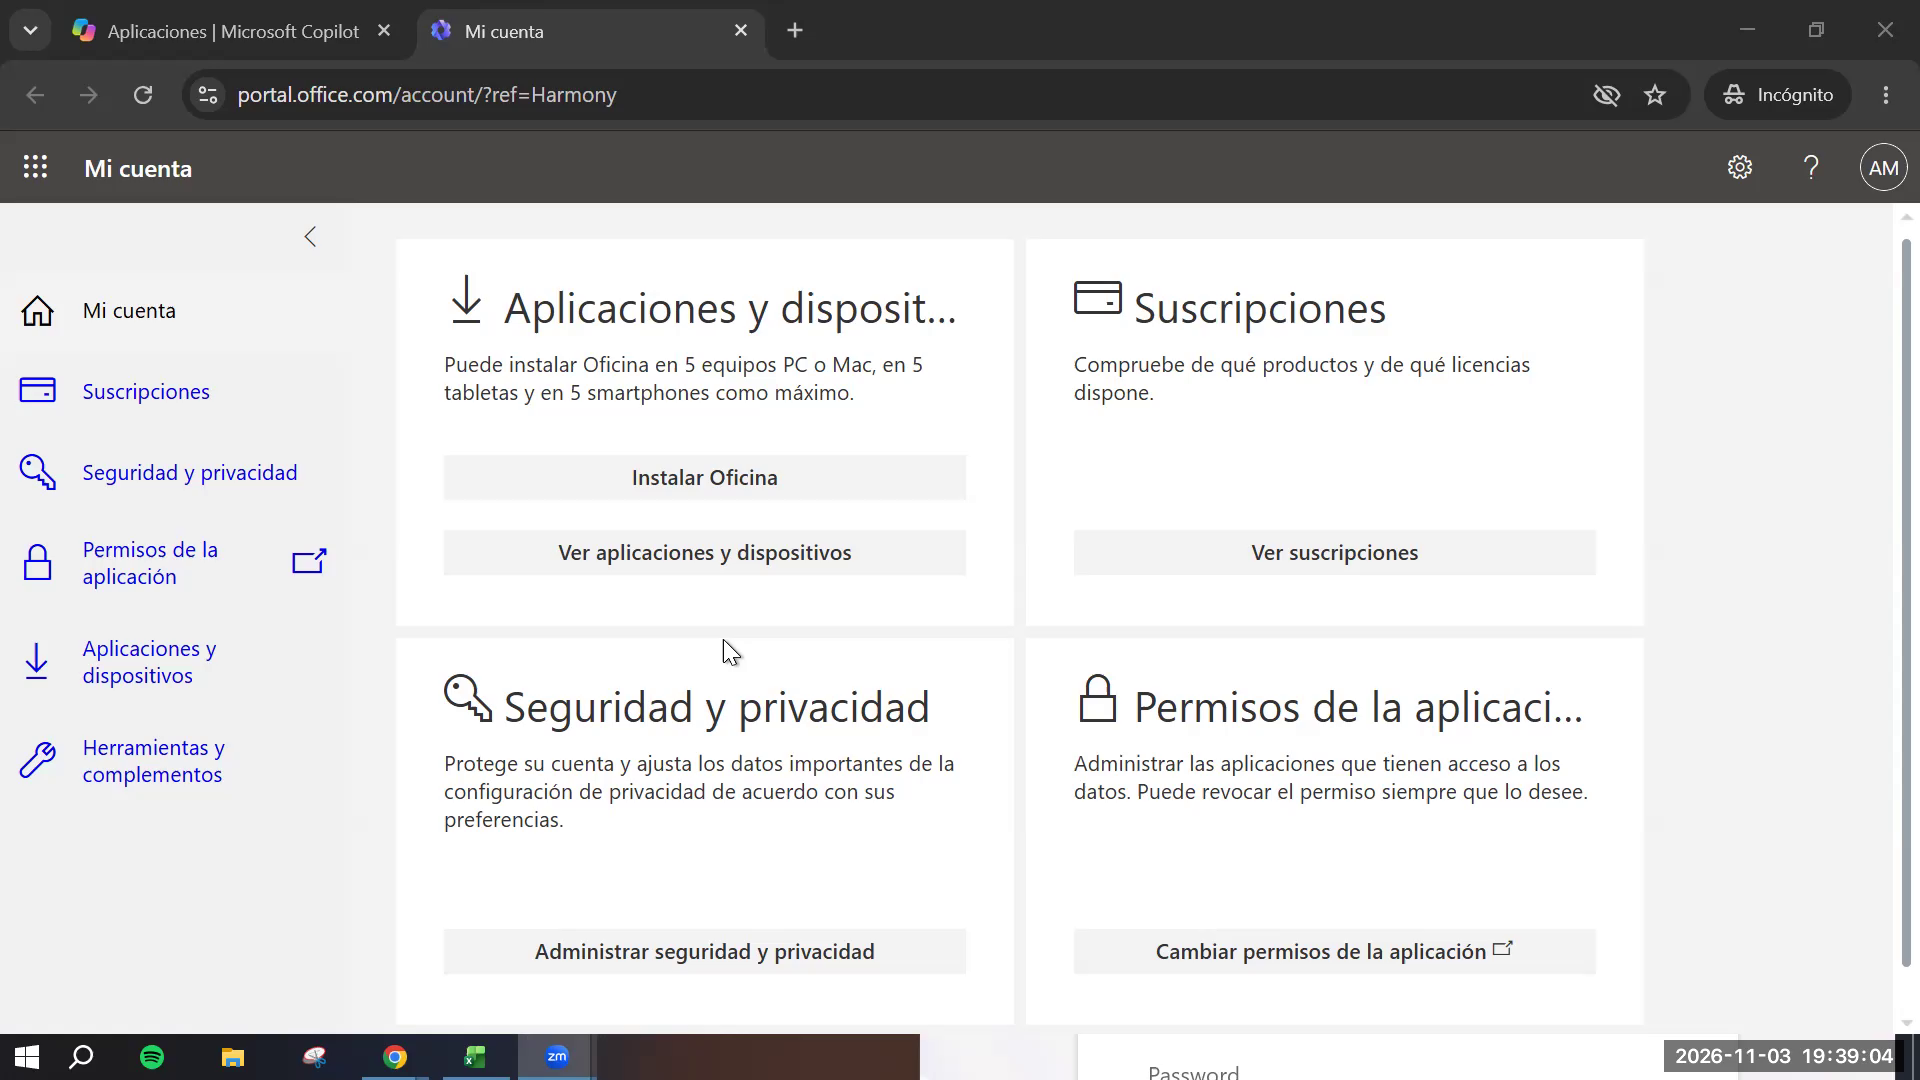
\includegraphics[width=0.88\linewidth]{referencias-herramientas-digitales/notas-herramientas-digitales/materiales-aula/capturas-clase/cap-16-s3-instalacion-activacion-m365-excel-00-21-15.png}
  \caption{Evidencia visual de clase [00:21:15]: Sesión guiada de la Semana 3 donde el docente asesora en pantalla la activación de cuenta Microsoft 365 y la instalación de Excel 365 con licencia institucional UAS. Fuente: Grabación docente UAS \cite{ruiz2026claseS1c1}.}
  \label{fig:uas-cap16-instalacion-m365}
\end{figure}
